% ============================================================================
% Chapter 7: Discussion and Conclusion
% Thesis: Pattern-Informed Fuzzy Deep Learning for Interpretable
%         Genotype–Phenotype Inference in Lung Adenocarcinoma
%         under Data Scarcity
% Author: Servio F. Lima
% University of Fribourg
% ============================================================================

\chapter{Discussion and Conclusion}
\label{ch:discussion}

This chapter discusses the implications, limitations, and contributions of the work presented in this thesis.
Section~\ref{sec:disc:contributions} synthesises the principal contributions.
Section~\ref{sec:disc:interpretation} interprets the results in the broader context of computational pathology and fuzzy soft computing.
Section~\ref{sec:disc:limitations} discusses the limitations.
Section~\ref{sec:disc:future} identifies directions for future work.
Section~\ref{sec:disc:conclusion} concludes the thesis.


% ============================================================================
\section{Summary of Contributions}
\label{sec:disc:contributions}
% ============================================================================

This thesis makes six contributions, each backed by specific
evaluation findings from Chapter~\ref{ch:evaluation}.
Table~\ref{tab:contribution_finding_map} summarises the mapping.

\begin{table}[ht!]
\centering
\small
\caption[Mapping of contributions to supporting implementation
and evaluation evidence]{Mapping of contributions to supporting
implementation and evaluation evidence. Numerical metrics and
RQ outcome verdicts are reported separately in
Table~\ref{tab:rq_summary_ch7} (Section~\ref{sec:disc:conclusion})
to keep the two tables orthogonal.}
\label{tab:contribution_finding_map}
\begin{tabular}{@{}c p{3.6cm} p{8.0cm}@{}}
\hline
\textbf{\#} & \textbf{Contribution} & \textbf{Supporting evidence} \\
\hline
C1 & FuzzyArcLoss~V2 (Artefact~1)
   & Impl.: Sec.~\ref{sec:impl:pattern}.\;
     Eval.: RQ1, Sec.~\ref{sec:eval:pattern:kfold} \\
C2 & PI-ABMIL (Artefact~2)
   & Impl.: Sec.~\ref{sec:impl:mutation}.\;
     Eval.: Finding~1 (RQ2(i)) and six-level XAI framework
     (RQ4); Sec.~\ref{sec:eval:interp:attention} \\
C3 & FC-MIL (Artefact~3)
   & Impl.: Sec.~\ref{sec:impl:choquet}.\;
     Eval.: Findings~2 and~6 (RQ2(i), RQ3);
     architectural negative control on RBM10
     (Sec.~\ref{sec:eval:interp:choquet}) \\
C4 & LCHAI~v2.0 prototype
   & Impl.: Sec.~\ref{sec:impl:lchai}.\;
     Eval.: Sec.~\ref{sec:eval:lchai}
     (end-to-end demo on the 6 representative TCGA-LUAD
     slides) \\
C5 & Mechanism-bound utility of fuzzy representations
   & Eval.\ only (analytical insight): Findings~3 and~4
     (RQ2(i), RQ2(ii)); per-slide ablation
     Tab.~\ref{tab:enrichment_summary} \\
C6 & Ontology explanation layer
   & Impl.: Sec.~\ref{sec:impl:ontology}.\;
     Eval.: RQ6, RQ7
     (Sec.~\ref{sec:eval:rq}) \\
\hline
\end{tabular}
\end{table}

\begin{figure}[ht!]
\centering
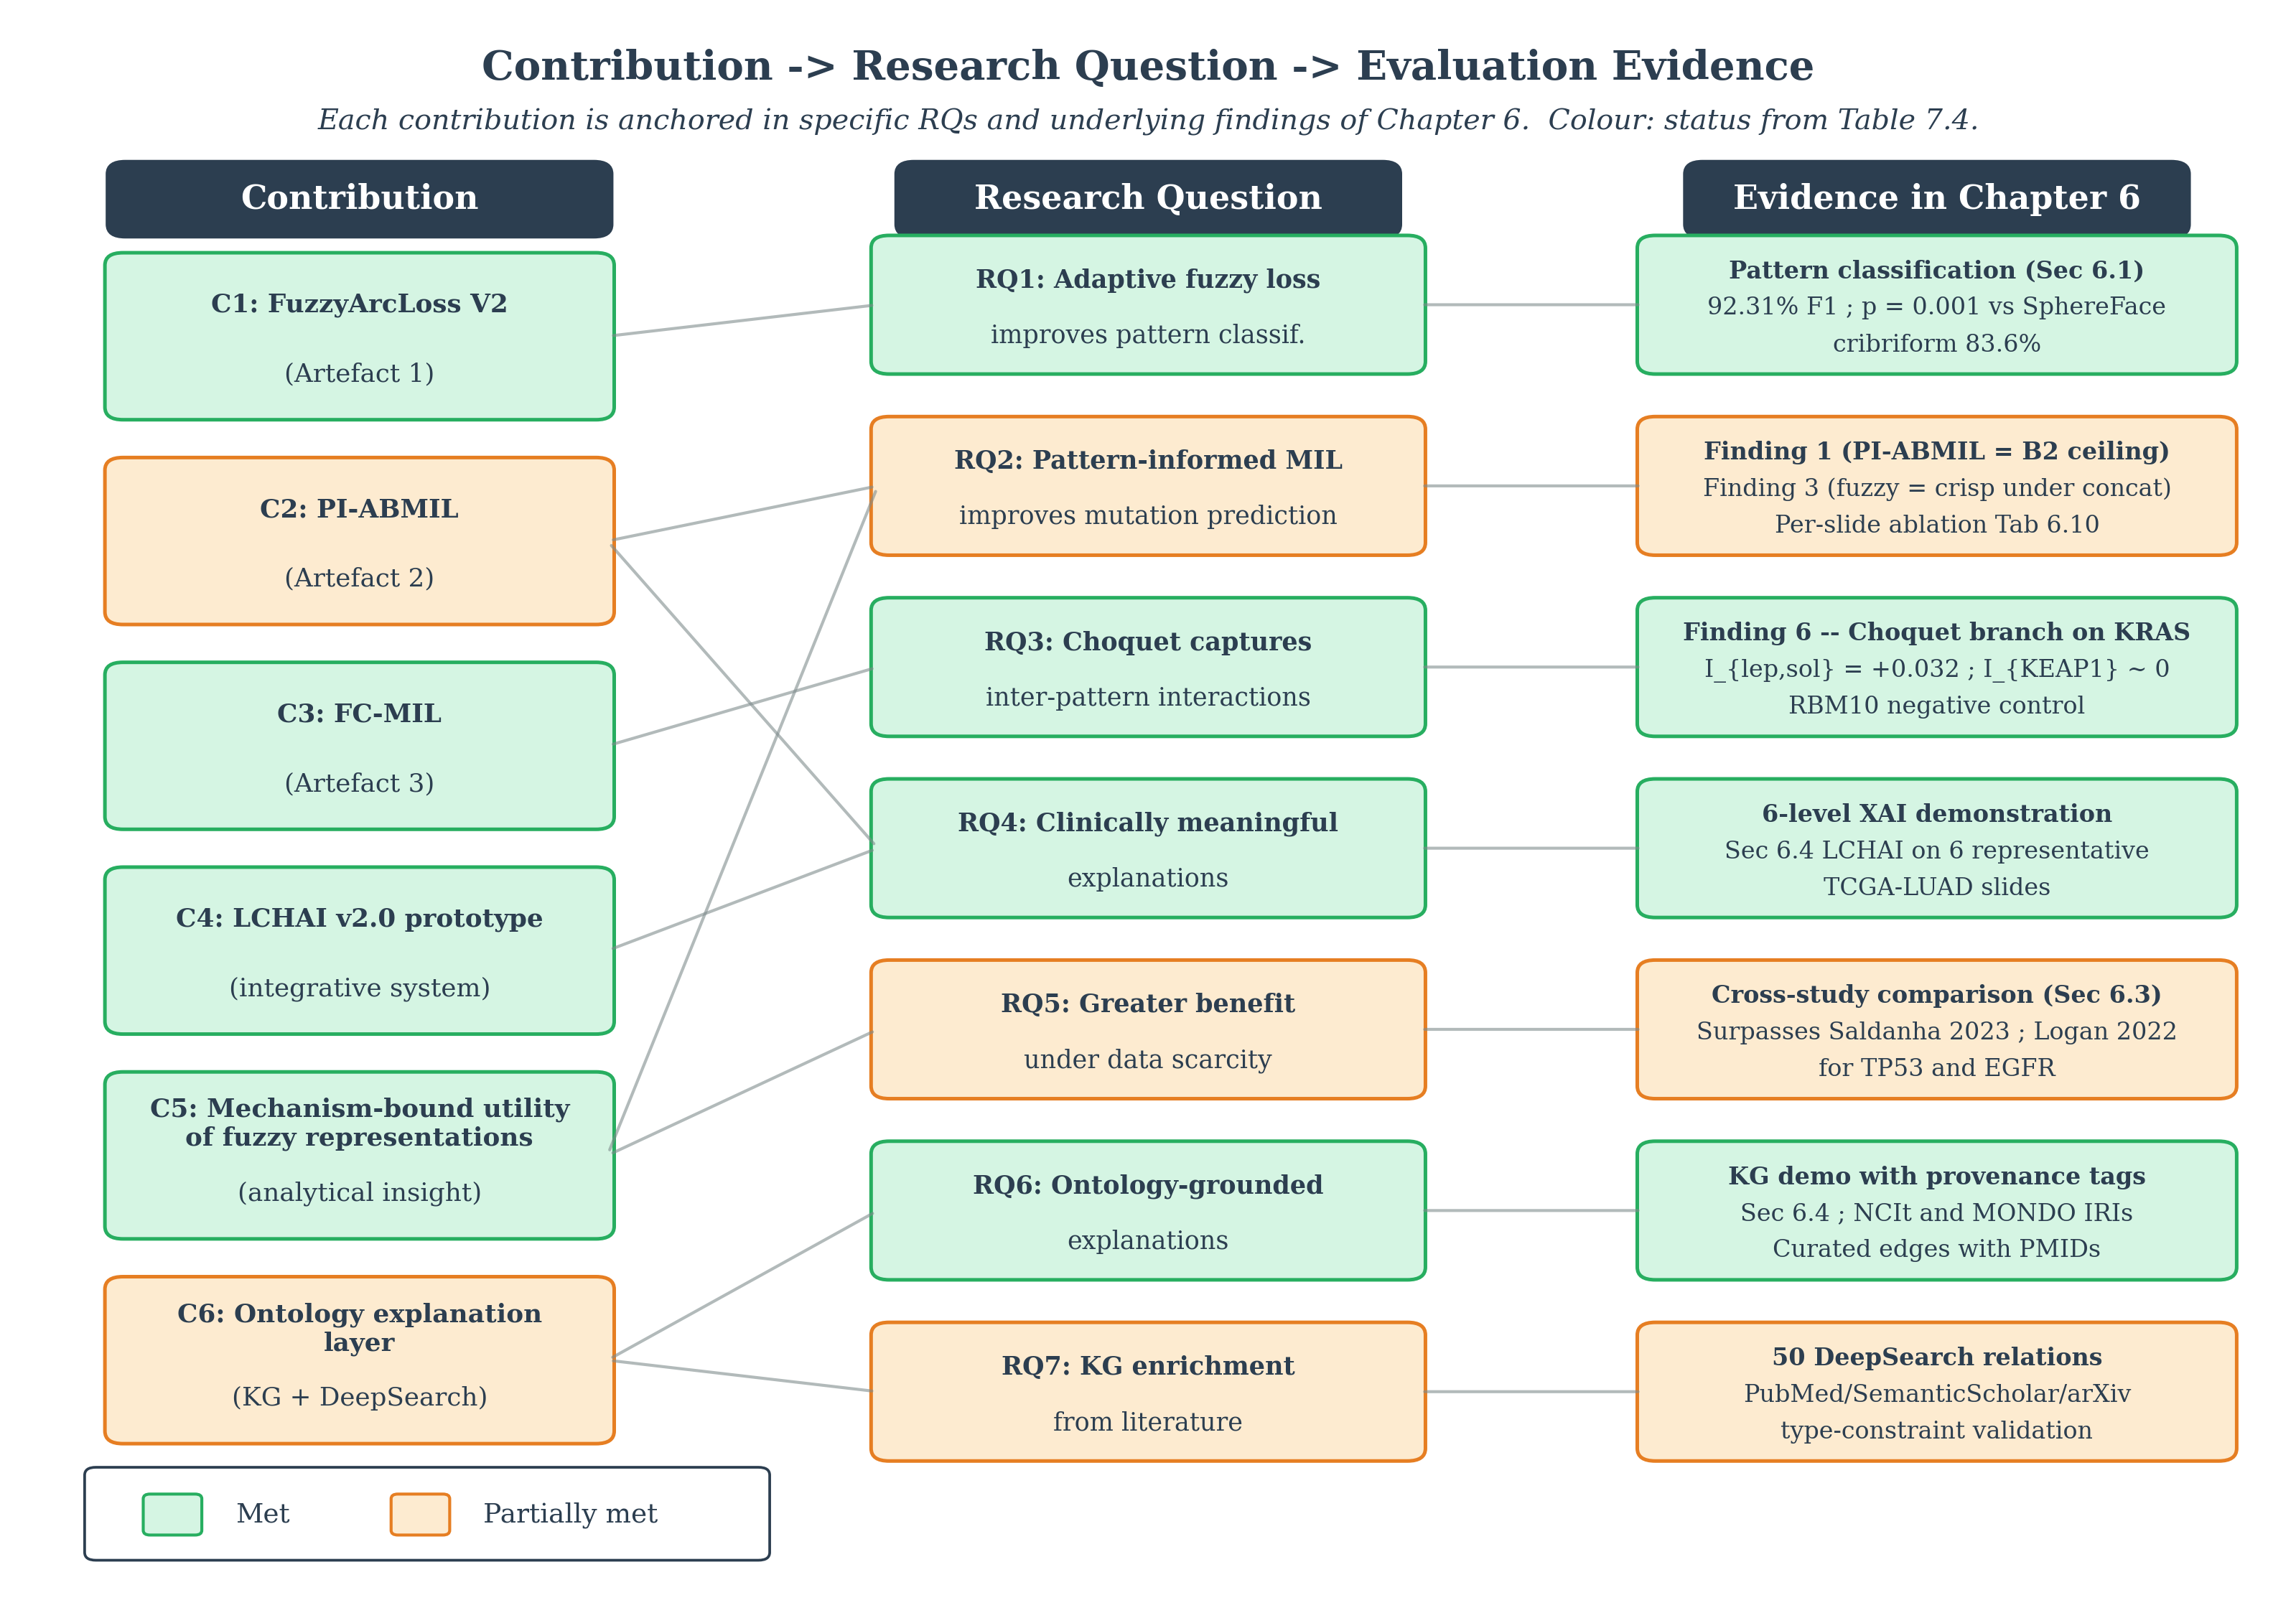
\includegraphics[width=\textwidth]{chapters/figures/contribution_evidence_map.png}
\caption[Contribution to evidence map]{%
    Three-column map of the discursive structure of the thesis.
    Each Contribution C1--C6 (left) is anchored in one or more
    Research Questions RQ1--RQ7 (centre), which in turn draw
    on specific Findings of Chapter~\ref{ch:evaluation}
    (right; figure references give the underlying numerical
    evidence).
    Colours follow Table~\ref{tab:rq_summary_ch7}: green = Met,
    amber = Partially met.
    Grey lines connect contributions to the RQs they answer and
    RQs to the supporting evaluation evidence.
    The map is the visual companion of
    Table~\ref{tab:contribution_finding_map}.}
\label{fig:contribution_evidence_map}
\end{figure}

\textbf{Contribution 1: FuzzyArcLoss V2 (Artefact 1).}
A novel angular margin loss with per-sample fuzzy-membership
modulation of the ArcFace
margin~\cite{deng2019arcface,wang2018cosface,liu2017sphereface},
allowing the loss to respect gradual morphological transitions
between pattern classes.
On the ANORAK 6-pattern benchmark FuzzyArcLoss~V2 ranks first among
18 compared loss functions ($p = 0.001$ vs.\ the strongest baseline;
Section~\ref{sec:eval:pattern:kfold}), and its advantage on the
ambiguous cribriform--acinar boundary
(``boundary'' here meaning the \emph{decision surface between
adjacent histological pattern classes}) is
\emph{morphological-boundary-dependent, not
class-size-dependent}---confirming that the fuzzy-margin
mechanism helps where adjacent classes overlap visually and
inter-annotator agreement is low, rather than where classes
have few training samples
(Section~\ref{sec:eval:pattern:perclass}).
The 20-pipeline-issues audit that fixed implementation drift
across all 18 baselines before the benchmark is documented in
Section~\ref{sec:meth:pattern:pipeline_audit}.

\textbf{Contribution 2: Pattern-Informed ABMIL (Artefact 2).}
A multiple-instance-learning aggregator that fuses CTransPath visual
embeddings with fuzzy pattern memberships, injecting validated
histological domain knowledge as a structured prior alongside the
learned visual features.
The architecture is the substrate for a six-level interpretability
framework formally defined in
Section~\ref{sec:meth:interpretability} and demonstrated on
representative TCGA-LUAD cases in
Section~\ref{sec:eval:interp:attention}, allowing a pathologist to
verify and critique the model's reasoning against the original
slide---a capability absent from prior end-to-end mutation
predictors.

\textbf{Contribution 3: Fuzzy Choquet MIL (Artefact 3).}
An aggregation mechanism that augments standard attention pooling
with a parallel Choquet-integral branch operating on tile-level
fuzzy pattern memberships under a \emph{learned 2-additive fuzzy
measure}.
The 2-additive restriction reduces the parameter count of a general
fuzzy measure on six sources from $2^6 - 2 = 62$ to $6 + 15 = 21$
(six singleton Shapley values plus fifteen pairwise interaction
indices) while still capturing the most informative pairwise
pattern synergies and redundancies.
FC-MIL is the sole top performer for \textit{KRAS} and
\textit{RBM10} (Section~\ref{sec:eval:interp:choquet}); the
\textit{KRAS} gain reflects a genuine inter-pattern interaction
(lepidic\,$\times$\,solid co-presence) that proxies the missing
invasive-mucinous class, whereas \textit{RBM10} serves as an
architectural negative control where the apparent lift originates in
the shared embedding pathway rather than the Choquet branch.

To the best of our knowledge, this is the first application of the
Choquet integral as a \emph{learned aggregation operator over
domain-specific semantic memberships} in computational pathology;
the differences from prior Choquet ensemble-fusion work
(\cite{bhowal2021fuzzybach}) and from the closest methodological
precedent (MICI~\cite{mccurley2023mici}) are detailed in
Section~\ref{sec:meth:choquet:motivation}.

\textbf{Contribution 4: LCHAI v2.0 Clinical Decision-Support
Prototype.}
An integrative system that wraps the three artefacts within a
unified clinical workflow, exposing the tile-level pattern
overlay, slide-level mutation prediction, a
\emph{cohort-level} Conclusive/Inconclusive reliability flag
(per-gene verdict on the held-out folds, not a per-slide score),
the six-level interpretability framework of Contribution~2, the
ontology-grounded knowledge graph of Contribution~6, and a dual
anti-hallucination mechanism (knowledge-graph grounding plus
fuzzy-label injection into LLM prompts) for clinician-readable
explanations.
End-to-end demonstration on six representative TCGA-LUAD slides is
reported in Section~\ref{sec:eval:lchai}.

\textbf{Contribution 5: Mechanism-Bound Utility of Fuzzy
Representations (Analytical Insight).}
The original analytical contribution is mechanism-bound rather than
gene-list-bound: the contrast between soft fuzzy probabilities and
hard one-hot labels becomes mechanically relevant only when the
aggregator can read \emph{joint} activations across channels
(Finding~3, Section~\ref{sec:eval:mutation:finding3}).
Within additive concatenation the two encodings are interchangeable
up to fold variance regardless of the underlying biology; only an
interaction-aware aggregator unlocks the discriminative content of
soft probabilities, and only for the gene whose biology lives in
inter-pattern co-occurrence.
Per-slide channel ablation
(Table~\ref{tab:enrichment_summary}) reinforces this finding at the
individual case level by dissociating feature \emph{attribution}
from predictive \emph{utility}: when no representation within the
ANORAK simplex recovers a discriminative signal, the cause is
biological---label-space
mismatch~\cite{lipton2018labelshift}, no morphological projection,
or collapse-to-prior~\cite{bowman2016posteriorcollapse}
(RQ2(ii), Section~\ref{sec:eval:rq2})---rather than architectural.
The contribution thus connects the biological nature of the
morphology--genotype relationship to the appropriate representation
\emph{and aggregation mechanism}, providing guidance for future
pattern-informed mutation prediction.

\textbf{Contribution 6: Ontology-Grounded Explanation Layer.}
A three-tier knowledge-graph architecture that links predicted
patterns and mutation hypotheses to standardised biomedical
ontologies (NCIt, MONDO) without influencing model training or
prediction.
The \emph{curated} layer encodes established evidence from
WHO~2021, OncoKB/FDA, TCGA/CIViC, and COSMIC as IRI-grounded
assertions with explicit provenance;
the \emph{dynamic} layer filters the graph per case to retain only
morphologically relevant entities;
the \emph{DeepSearch} layer continuously mines PubMed, Semantic
Scholar, and arXiv for candidate pattern--mutation--treatment
relations subject to type-constraint validation.
The combination provides ontology-grounded, auditable explanations
(RQ6) and continuous knowledge enrichment (RQ7)---capabilities
absent from prior H\&E-based mutation prediction methods.
% ============================================================================
\section{Interpretation of Results}
\label{sec:disc:interpretation}
% ============================================================================
\subsection{On the Role of Domain Knowledge Under Data Scarcity}
\label{sec:disc:interp:domain}

The central hypothesis of this thesis
(Section~\ref{sec:intro:hypothesis}) makes two conjoined claims:
that \emph{structured} domain knowledge---expert-defined
histological growth patterns encoded through fuzzy set
theory---can be injected into a deep-learning mutation prediction
pipeline to simultaneously (a)~achieve \emph{competitive}
predictive performance under data scarcity ($<$\,700 public
slides), and (b)~render the resulting predictions
\emph{interpretable} through a multi-level, clinically verifiable
inspection framework---and, through that framework,
\emph{explainable} via knowledge-graph--grounded natural-language
rationales---to a degree that no end-to-end black-box approach
offers (Section~\ref{sec:bg:xai:definitions}).
This subsection examines clause~(a); clause~(b) is the subject of
the interpretability--performance trade-off in
Section~\ref{sec:disc:interp:tradeoff}.
The empirical results support clause~(a) \emph{partially and
mechanism-conditionally}, and the nature of that partial support
is itself informative.

At the cohort level, Pattern-Informed ABMIL matches the
embedding-only ceiling baseline (B2) in mean AUROC (both
0.658) but does not exceed it: the CTransPath encoder, pretrained
on ${\sim}15$~million histopathology tiles, already encodes
morphological information that largely subsumes the six-pattern
ANORAK taxonomy under additive concatenation, so the explicit
pattern channel is marginally redundant for \emph{prediction} when
the aggregator simply concatenates the two views.
At the per-slide level the picture is sharper: the pattern channel
helps only for KRAS, is informationally redundant for the
representative EGFR slide, hurts predictions for TP53, STK11, and
KEAP1, and drives RBM10 into a collapse-to-prior null regime
(Table~\ref{tab:enrichment_summary},
Figure~\ref{fig:signal_tree}).
Crucially, the pattern channel remains essential for
\emph{interpretability}---even when patterns hurt prediction, their
presence enables the system to \emph{explain why} they hurt
(false-positive attribution, attention on decoy regions, or
collapse-to-prior).

The KRAS case isolates the mechanism by which the pattern prior
yields \emph{predictive} value over a strong pretrained encoder.
Within additive concatenation (PI-ABMIL) the fuzzy and crisp
encodings of the same six pattern channels are interchangeable up
to fold variance for all six genes (Finding~3,
Section~\ref{sec:eval:mutation:finding3}); the soft-vs-hard
distinction becomes mechanically relevant only when the aggregator
can read \emph{joint} activations across channels, as in FC-MIL,
where the learned 2-additive Choquet measure picks up the
lepidic\,$\times$\,solid co-presence as a proxy for the missing
invasive-mucinous class.
On RBM10---where FC-MIL also outperforms ABMIL at the cohort
level---the Choquet branch is empty (singleton-only measure with
near-zero pairwise interactions) and the apparent lift originates
in the shared embedding pathway, so RBM10 functions as an
architectural negative control rather than as a second example of
pattern-level signal
(Section~\ref{sec:eval:interp:choquet}).

These observations point to a narrower conclusion than the common
``small model with domain prior beats large model'' narrative:
\emph{the pattern prior gives a predictive advantage over a
strong pretrained encoder only when (i)~the aggregator can read
joint activations across pattern channels, and (ii)~the target
gene's biology lives in inter-pattern co-occurrence rather than in
a single dominant correlate.}
Outside that regime---when a gene's dominant correlate is already
encoded in the pretrained features (TP53, EGFR), or when no
representation within the ANORAK simplex recovers any
discriminative signal at all (STK11, KEAP1, RBM10; three-mechanism
RQ2(ii) taxonomy)---additional pattern information becomes
redundant or actively interferes with prediction, while still
providing a transparent failure trace.
Whether the pattern prior would yield a broader advantage in
settings with substantially fewer slides per gene ($N \ll 500$) or
with weaker pretrained encoders is a plausible but \emph{untested}
hypothesis: the dominant axis of variation in the per-slide
ablation of this thesis is gene biology rather than sample size,
so direct verification would require either a small institutional
cohort or an encoder ablation that replaces CTransPath with a
smaller in-domain model---both noted as future work
(Section~\ref{sec:disc:future:medium}).


\subsection{On the Interpretability--Performance Trade-Off}
\label{sec:disc:interp:tradeoff}

The H\&E mutation prediction literature surveyed in
Section~\ref{sec:bg:related} traces an inverse relationship between
cohort scale and interpretability: each generation
(Coudray~2018~$\to$~Saldanha~$\to$~DeepGEM/EAGLE/CHIEF) raises both
$N$ and architectural complexity while reducing the granularity
at which a pathologist can verify individual predictions.
Figure~\ref{fig:interpretability_vs_data_scale} visualises this
trajectory; the formal numerical comparison is in
Section~\ref{sec:eval:literature}.

\textbf{This thesis charts an alternative course at zero net
cohort-level cost.}
PI-ABMIL ties the embedding-only ceiling B2 on cohort mean AUROC
(Finding~3, Section~\ref{sec:eval:mutation:finding3}) and, within
the public-data regime, statistically matches
Saldanha~et~al.~\cite{saldanha2023npj} and
Logan~et~al.~\cite{logan2022medrxiv} on TP53 and EGFR
(Section~\ref{sec:eval:literature}), so the addition of an
inspectable pattern channel \emph{costs no AUROC} relative to
public-data peers.
The gap to foundation-scale studies (DeepGEM, EAGLE, CHIEF) tracks
the public-vs-proprietary data asymmetry on a log axis---a
structural cohort-size effect, not a methodological ceiling
(Figure~\ref{fig:interpretability_vs_data_scale}).

\begin{figure}[ht!]
\centering
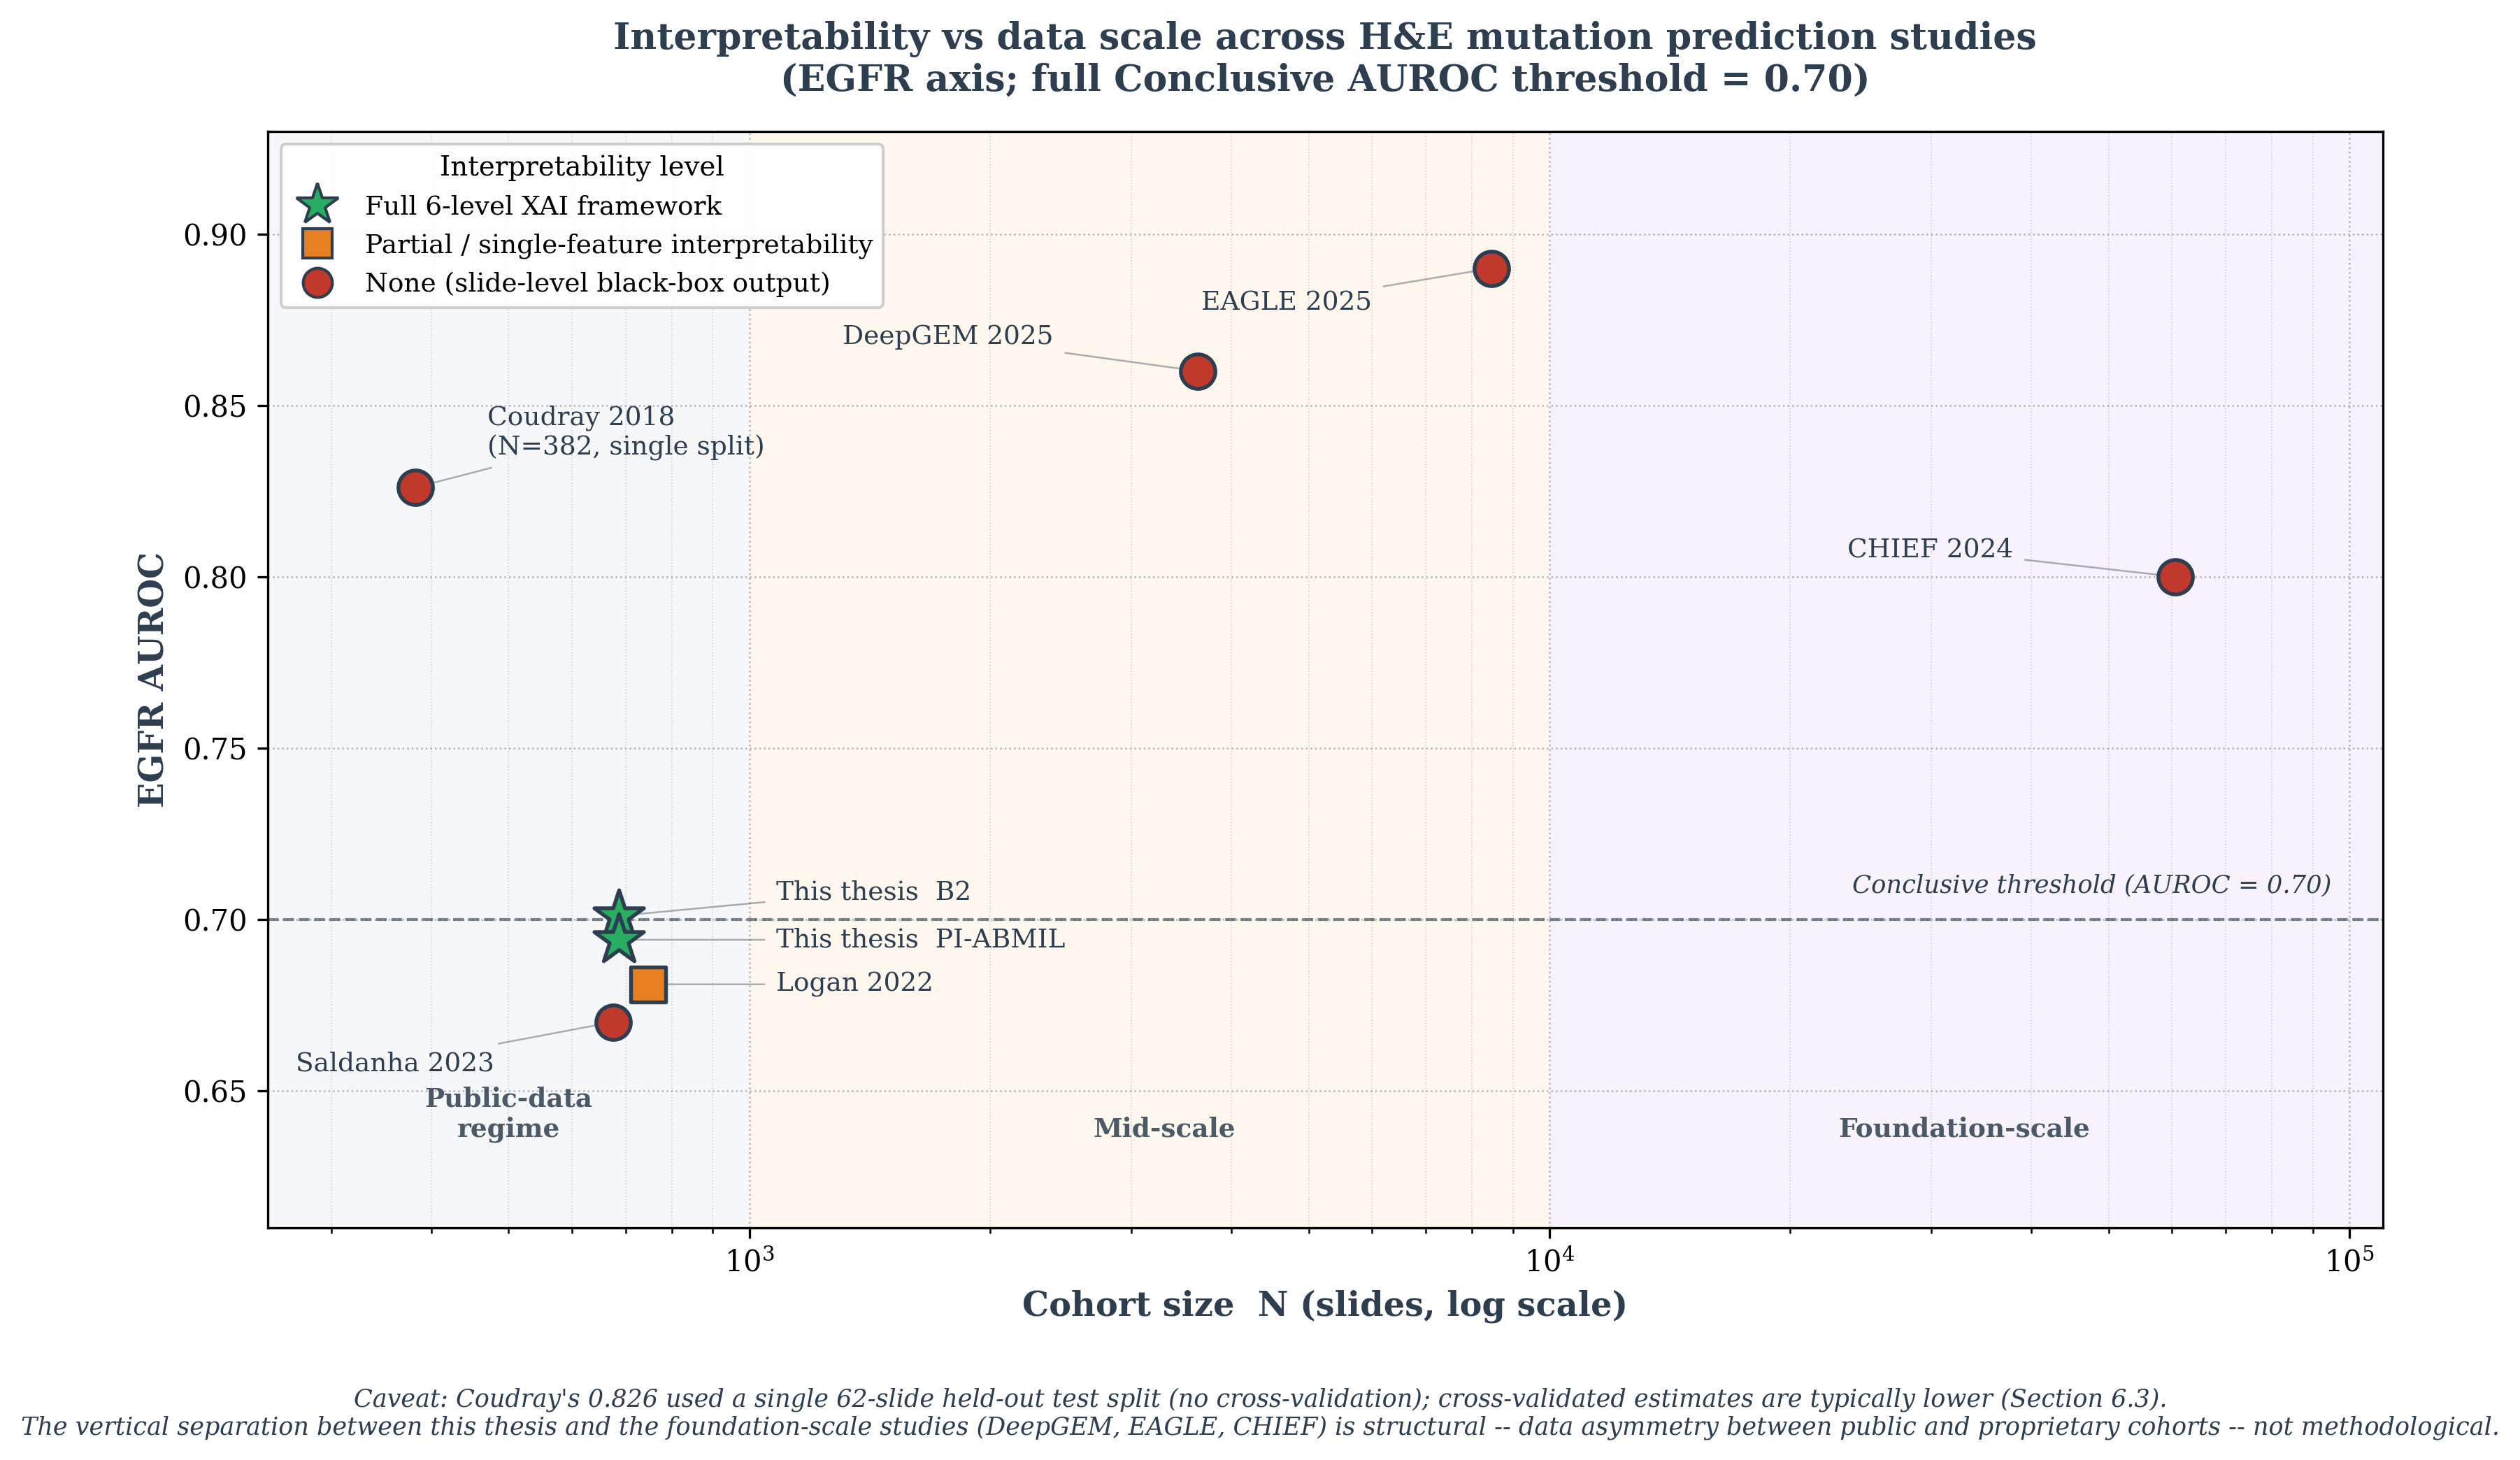
\includegraphics[width=\textwidth]{chapters/figures/interpretability_vs_data_scale.png}
\caption[Interpretability vs data scale across published studies]{%
    EGFR AUROC plotted against cohort size $N$ (log scale) for
    published H\&E mutation prediction studies. Marker shape and
    colour encode the level of interpretability the system
    offers (full 6-level XAI framework, partial / single-feature
    interpretability, or none). The dashed line marks the
    Conclusive AUROC threshold of $0.70$. Background bands
    distinguish three data regimes: public-data ($N \approx
    400$--$1\,000$), mid-scale ($1\,000$--$10\,000$) and
    foundation-scale ($>10\,000$). Visual companion to the
    literature comparison of
    Section~\ref{sec:eval:literature}: the vertical separation
    from DeepGEM/EAGLE/CHIEF reflects public-vs-proprietary
    cohort asymmetry, while within the public regime this thesis
    sits above Saldanha~et~al.\ and Logan~et~al.\ at a strictly
    stronger interpretability tier.}
\label{fig:interpretability_vs_data_scale}
\end{figure}

\textbf{The cohort mean hides a gene-specific structure that
interpretability turns into a feature, not a bug.}
The per-slide ablation (Table~\ref{tab:enrichment_summary},
Section~\ref{sec:eval:interp:enrichment}) shows that the
pattern-channel benefit is positive on KRAS, redundant on the
representative EGFR slide, and \emph{negative} on TP53, STK11 and
KEAP1 at the individual-case level---structure invisible at the
cohort-mean grain and routinely missed by black-box AUROC
benchmarks.
The same Level-5 ablation that exposes a negative
$\Delta_{\mathrm{pat}}$ also \emph{explains} it
(false-positive attribution, decoy-region attention, or
collapse-to-prior; representative cases worked out in
Section~\ref{sec:eval:interp:attention}).
Failure traces of this kind are absent from every black-box
predictor in the literature regardless of its headline AUROC.

\textbf{The trade-off is quantifiable but framed against design
objectives, not absolute AUROC.}
In the Design Science Research frame adopted in
Chapter~\ref{ch:methodology}, artefacts are evaluated against
their stated design objectives---interpretability, robustness to
data scarcity, principled integration of domain knowledge---rather
than against absolute AUROC rankings; against those criteria all
three artefacts meet or partially meet their success criteria
(Section~\ref{sec:eval:rq}).
Within that frame, three structural advantages of the proposed
approach over current foundation-scale competitors are not
captured by AUROC and merit explicit naming:
\begin{itemize}
  \item \textbf{Multi-level interpretability.} Where DeepGEM,
        EAGLE, CHIEF and GigaPath~\cite{zhao2025deepgem,%
        campanella2025eagle,wang2024chief,xu2024gigapath} expose
        a single mutation probability, LCHAI~v2.0 exposes the
        six-level XAI stack of Contribution~2
        (Section~\ref{sec:meth:interpretability};
        demonstrations in Section~\ref{sec:eval:lchai}).
  \item \textbf{Gene-dependent aggregator selection.} LCHAI
        selects the per-gene best-in-expectation aggregator
        (Finding~2, Section~\ref{sec:eval:mutation:finding2}); the
        biological reasoning behind the per-gene choices is
        developed in Section~\ref{sec:disc:interp:domain}.
        Foundation-scale systems apply a single architecture
        uniformly to all genes.
  \item \textbf{Intrinsic interpretability and full
        reproducibility.} FC-MIL's 21-parameter learned fuzzy
        measure yields intrinsic Shapley-value attribution
        (Contribution~3) that no attention-based aggregator
        provides; all results in this thesis are reproducible
        from public TCGA-LUAD slides with public code, in
        contrast to proprietary-data systems whose results
        cannot be externally verified.
\end{itemize}


\subsection{On the Genotype--Phenotype Mismatch}
\label{sec:disc:genotype_phenotype}

A recurrent finding throughout the evaluation is a structural
asymmetry in the error distribution: the failure cases are
predominantly \emph{false negatives} where the binary mutation
label is positive (confirmed by DNA sequencing) but the predicted
probability is low because the slide's morphology---and, by
extension, its pretrained embedding---falls outside the region of
feature space that the population-level training signal associates
with the mutated class.
The EGFR case TCGA-86-8280 (Section~\ref{sec:eval:interp:attention})
is a clear example.
At the population level EGFR is Conclusive (cohort 5-fold
AUROC~$= 0.701$, B2 embeddings); the individual slide receives
P(mut)~$= 0.076$ despite being 94.9\% micropapillary with very
little of the canonical EGFR-associated patterns (lepidic 0.3\%,
papillary 0.05\%), placing it in the left tail of the
EGFR-mutant score distribution where atypical-morphology positives
are expected to fall (Figure~\ref{fig:egfr_score_overlap}).
The failure is therefore not that the model lacks the pattern
channel---the prediction is from the embedding-only ceiling
baseline B2, which does not use patterns at all---but that the
slide's embedding lies in a region of feature space the
EGFR-mutant cohort underpopulates: a statistically expected
false negative that the per-slide pattern overlay then
\emph{annotates} (94.9\% micropapillary, near-absent
lepidic/papillary) without participating in the prediction.

From a learning standpoint, the underlying issue is that the
mapping from genotype to phenotype that the model is asked to
invert is fundamentally \textbf{stochastic, many-to-many, and
weakly labelled}---not a deterministic function.
Where the structural RQ2(ii) taxonomy of
Section~\ref{sec:eval:rq2} classifies \emph{genes} by whether any
representation within the ANORAK simplex recovers a discriminative
signal, the taxonomy below classifies \emph{failure modes} by
\textbf{where in the input--label information chain
(DNA $\rightarrow$ protein $\rightarrow$ tissue $\rightarrow$
sequenced fragment $\rightarrow$ model output) the signal is
lost or the label is decoupled from the feature}.
Figure~\ref{fig:genotype_phenotype_mismatch} consolidates the four
mechanisms in a single view, mapping each to a point along the
chain at which information is lost:

\begin{figure}[ht!]
\centering
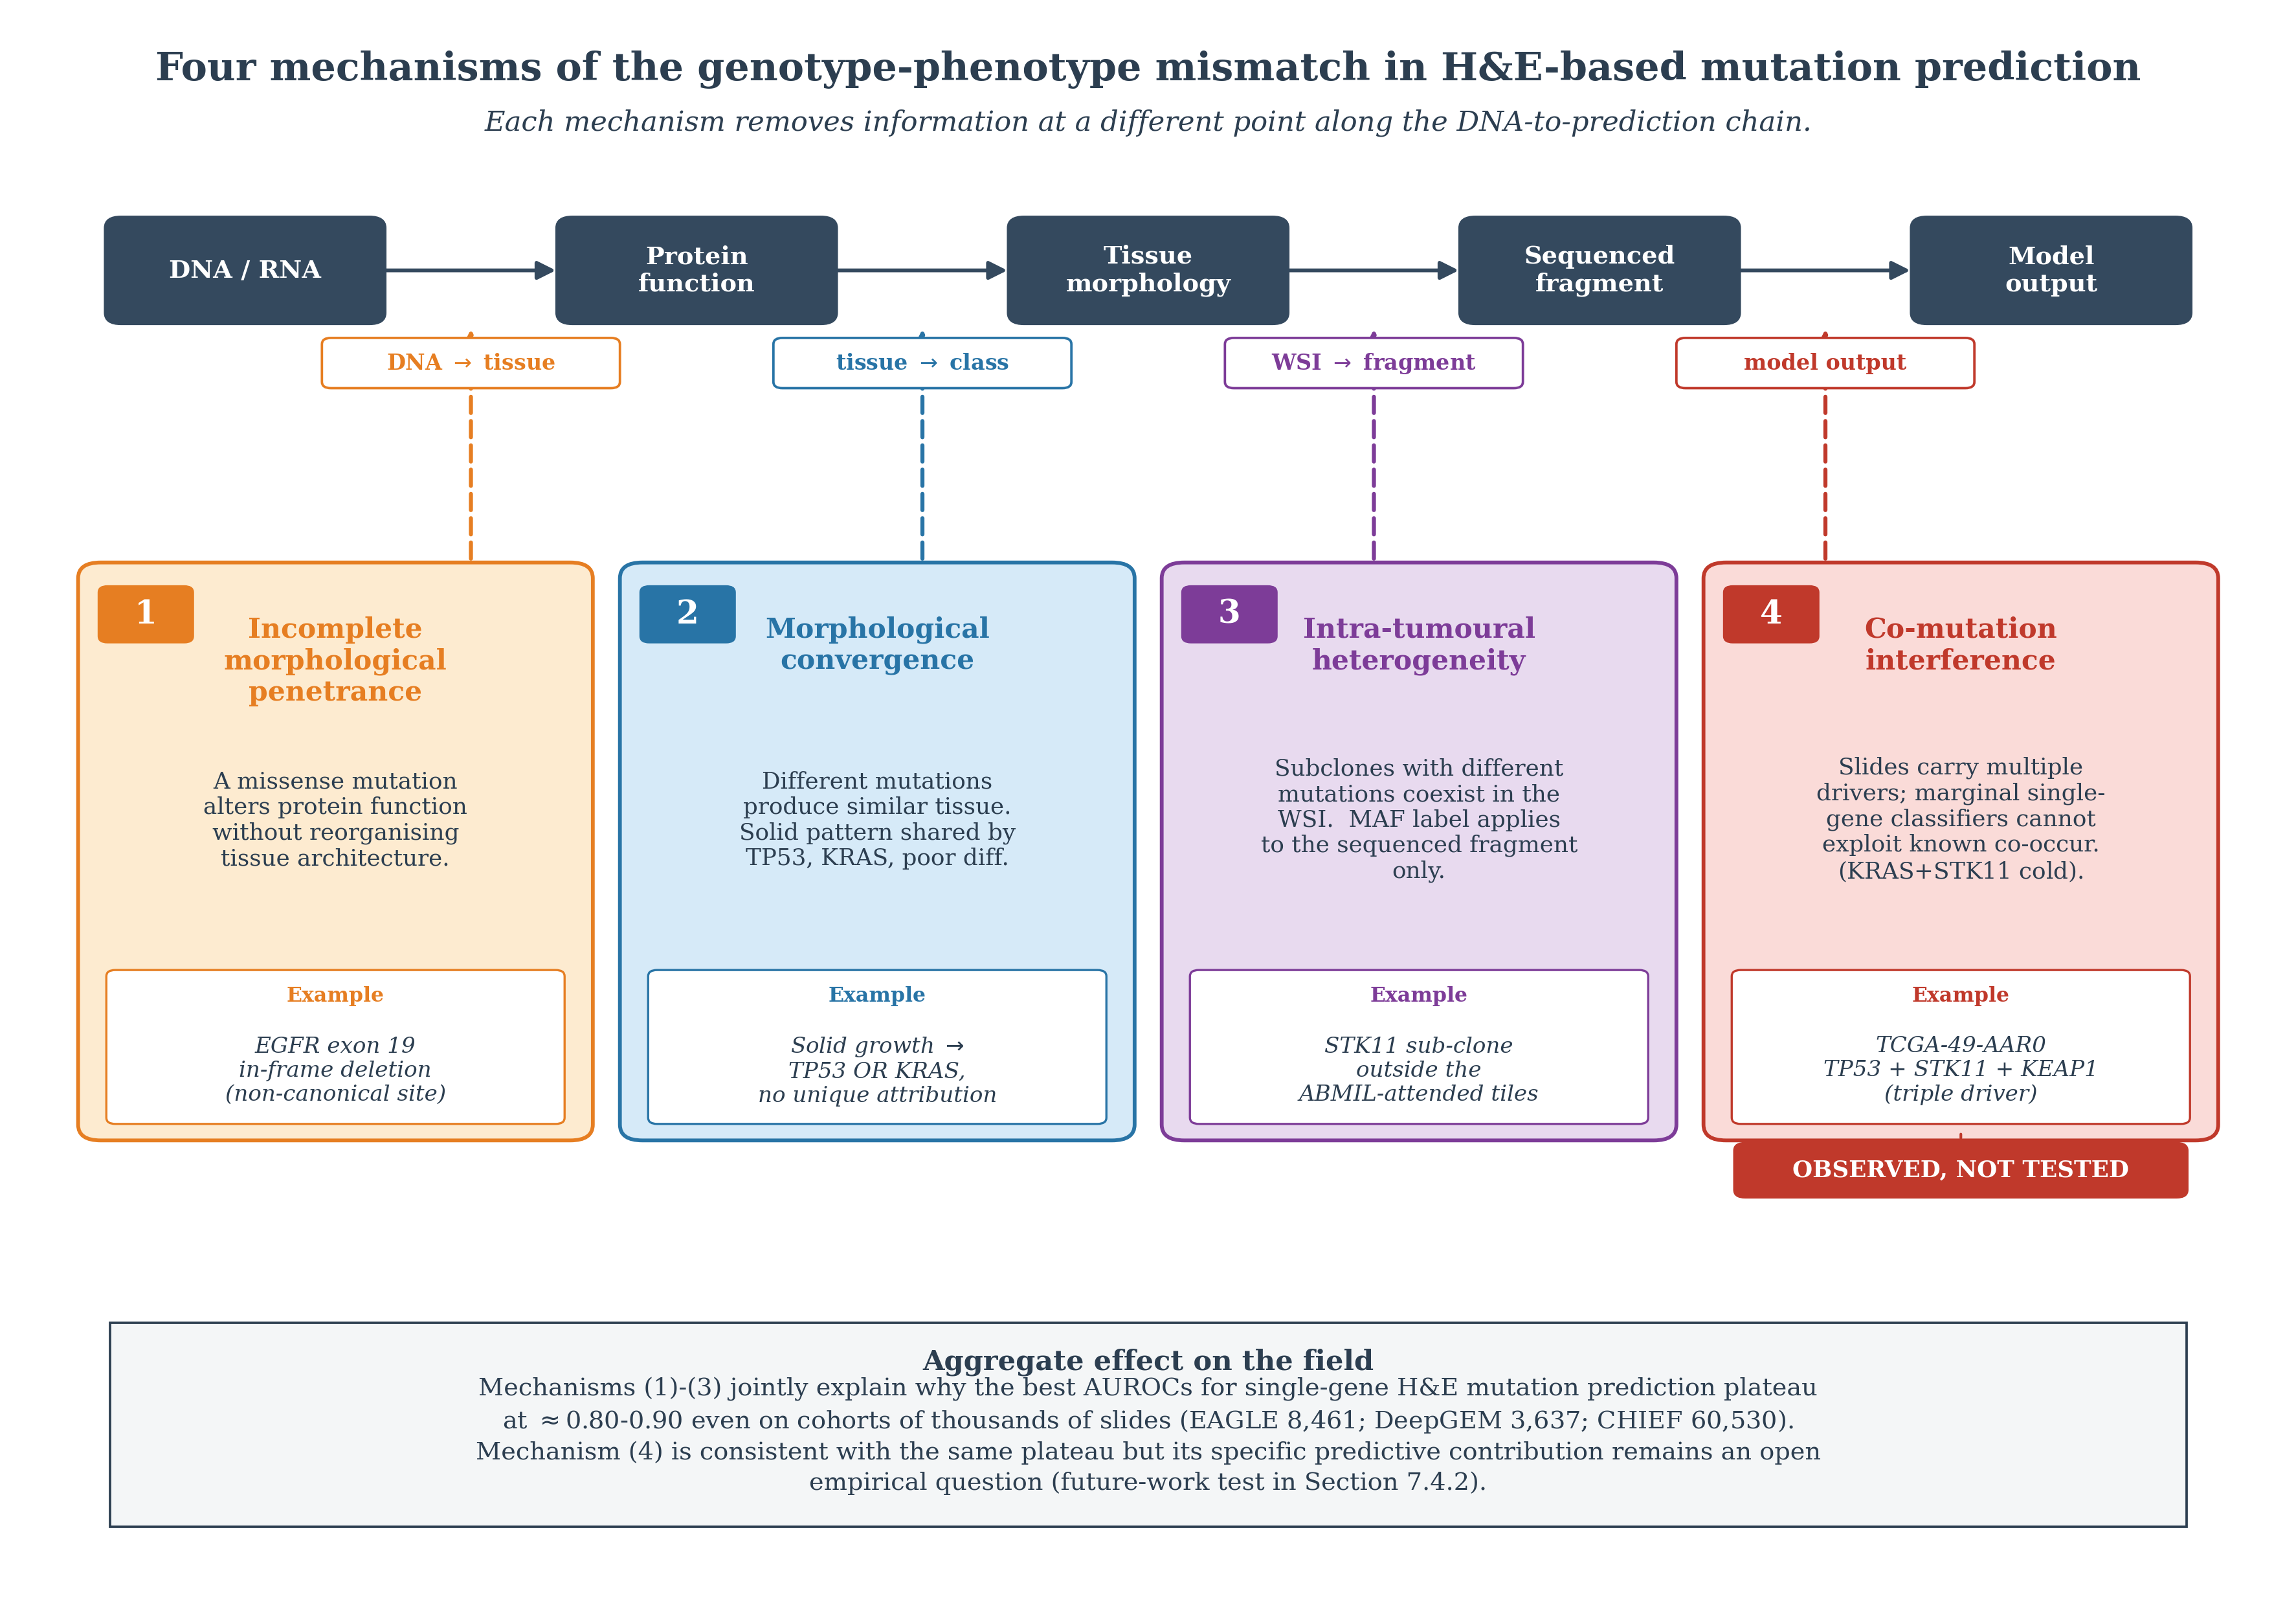
\includegraphics[width=\textwidth]{chapters/figures/genotype_phenotype_mismatch.png}
\caption[Four mechanisms of the genotype--phenotype mismatch]{%
    Four mechanisms of the genotype--phenotype mismatch in
    H\&E-based mutation prediction. The top spine traces the
    information-flow chain from genotype to model output (DNA
    $\rightarrow$ protein $\rightarrow$ tissue $\rightarrow$
    sequenced fragment $\rightarrow$ model output); each panel
    is a mechanism that removes information at one of the
    arrows of this chain.
    Examples are drawn from the case studies of
    Chapter~\ref{ch:evaluation}
    (Table~\ref{tab:enrichment_summary}).
    The bottom band reports the aggregate consequence: even
    foundation-scale studies plateau at AUROC
    $\approx 0.80$--$0.90$, reflecting an irreducible information
    gap between DNA and H\&E.}
\label{fig:genotype_phenotype_mismatch}
\end{figure}

\begin{enumerate}
    \item \textbf{Information loss at the source signal
    (incomplete morphological penetrance).}
    The first failure mode is information loss before the visual
    signal even forms.
    A mutation that alters protein function without reorganising
    cellular growth patterns leaves the H\&E appearance
    indistinguishable from wild-type tissue---i.e., the input
    that the encoder sees does not carry a discriminative
    feature, regardless of how powerful the encoder is.
    The effect is gene-region-dependent: the canonical
    EGFR-associated lepidic signature is driven specifically by
    exon~19 deletions and the L858R substitution (the
    terminal-respiratory-unit
    phenotype~\cite{yatabe2005egfrlepidic}), whereas uncommon
    EGFR variants display heterogeneous histology and a different
    therapeutic response
    profile~\cite{brindel2020uncommonegfr}.
    Within a single binary EGFR-mutated label, the canonical and
    uncommon variants are pooled, and the share of slides with no
    morphological footprint sets a lower bound on the
    achievable error rate.

    \item \textbf{Many-to-one mapping from genotype to morphology
    (morphological convergence).}
    The second failure mode is a fundamental ambiguity in the
    inverse problem the model is asked to solve.
    Different driver mutations can produce indistinguishable
    tissue phenotypes: the solid growth pattern, for example, is
    documented as a correlate of both
    TP53~\cite{ahn2022tp53highgrade} and
    KRAS~\cite{rekhtman2013krassolid}, and is itself a marker of
    poor differentiation in the WHO/IASLC
    grading~\cite{who2021thoracic,moreira2020ialcslurp}.
    A single-gene binary classifier observing a high-solid slide
    therefore faces a many-to-one mapping for which no purely
    visual posterior can be sharper than the prior over
    competing genes that share that pattern.

    \item \textbf{Weak slide-level labels and intra-tumoural
    heterogeneity.}
    The third failure mode is on the label side rather than the
    feature side, and stems from the way TCGA mutation labels are
    produced.
    Two heterogeneity layers compound: first, a single resected
    LUAD specimen typically contains a mixture of two or more
    growth
    patterns~\cite{warth2012interobserver,moreira2020ialcslurp},
    so the morphologically dominant region need not be the one
    that drives prognosis or carries the molecular signature of
    interest;
    second, the slide-level mutation label is derived from the
    MAF call on the \emph{sequenced fragment}---typically a
    macrodissected region whose tissue is consumed in the
    extraction step~\cite{gdc2024maf}---and is then assigned to
    the entire WSI as a single binary label, even when the
    mutated cells may occupy only part of the tumour.
    From a learning-theory standpoint this is a weak-label
    setting where the slide-level supervision is partially
    decoupled from the local tissue features the MIL aggregator
    actually attends to.

    \item \textbf{Independent-binary factorisation of a structured
    label space (co-mutation interference)}
    \emph{[observed in the cohort statistics of this thesis but
    not empirically tested; included for taxonomic completeness
    and as the motivation for a specific future-work
    experiment].}
    The fourth failure mode is on the label side and is
    architectural rather than data-side.
    Each gene is currently predicted by an independent binary
    classifier with its own loss; the joint label
    $\mathbf{y} \in \{0,1\}^6$ is factorised as the product of
    six marginals.
    The MAF analysis of the representative slides
    (Table~\ref{tab:enrichment_summary}) shows that this
    factorisation is at odds with the data: all six slides carry
    at least one additional driver mutation beyond the target
    gene, and four of six carry two or more co-mutations.
    The tissue morphology of a co-mutated tumour is, in principle,
    a superposition of the phenotypic effects of all its
    drivers---e.g.\ the clinically recognised KRAS--STK11
    immune-cold phenotype~\cite{skoulidis2018stk11pd1,%
    skoulidis2015krassubsets}---but the marginal classifiers
    used here cannot exploit such co-occurrence patterns by
    construction.
    Whether this architectural choice actually degrades
    predictive performance, and by how much, is the question that
    a multi-task vs single-task ablation would settle; that
    experiment is proposed in
    Section~\ref{sec:disc:future:medium} (``Multi-task and
    multi-gene learning'') rather than executed here.
    The other three mechanisms above are also primarily
    documented rather than ablated, but each is anchored in an
    independent observation visible in the case studies of
    Chapter~\ref{ch:evaluation}; mechanism~(4) is the only one
    whose predictive consequence has a clean, scoped empirical
    test that this thesis did not run.
\end{enumerate}

Together, mechanisms~(1)--(3) constitute a documented
\emph{structural} explanation of why the best-reported AUROCs for
single-gene mutation prediction from H\&E histology plateau around
0.80--0.90 even with proprietary datasets of thousands of slides
(Section~\ref{sec:eval:literature}); mechanism~(4) is consistent
with the same plateau but its specific contribution remains an
open empirical question.
On the strength of (1)--(3) alone, the residual 15--20\% error
rate is best read as an irreducible information gap between what
DNA sequences reveal and what tissue architecture shows, rather
than as headroom that better optimisation could close.

The four-mechanism taxonomy is rarely activated in isolation: every
representative slide carries at least one co-mutation and four of
six carry two or more, so the EGFR case above is simultaneously
consistent with mechanism~(2) (atypical embedding fingerprint) and
mechanism~(4) (co-mutation interference).
This co-incidence is exactly what motivates the multi-task
extension proposed in
Section~\ref{sec:disc:future:medium}; we do not re-propose it
here.


\subsection{On the Relationship Between Fuzzy Logic and Biological Gradience}
\label{sec:disc:interp:fuzzy}

A recurring theme throughout this thesis is the use of fuzzy set
theory as a principled treatment for \emph{label noise from
genuine class overlap}.
The six histological patterns of LUAD are not separable by sharp
decision surfaces in pixel space: many tiles fall on smooth
manifolds between two adjacent classes (e.g., acinar
$\leftrightarrow$ papillary), and expert agreement on those
boundary tiles is itself low (inter-observer
$\kappa \approx 0.38$~\cite{thunnissen2012reproducibility}).
The standard pipeline for tile classification collapses each tile
into a one-hot $\arg\max$ assignment and minimises a softmax
cross-entropy against it, which discards the boundary information
twice: once at labelling time (the annotator picks one class), and
again at training time (the loss treats the picked class as
ground truth).
Fuzzy set theory replaces the one-hot $\{0,1\}^6$ target with a
continuous $\Delta^5$ membership vector, making boundary
uncertainty a first-class quantity that propagates through the
pipeline rather than a quantisation error to be tolerated.

FuzzyArcLoss~V2 explicitly models this gradience at two levels.
At the training level, the fuzzy membership function reduces the angular margin for samples at pattern boundaries, preventing the model from overfitting to the assigned discrete label.
At the output level, the soft probability vector $\mathbf{p}_i \in \Delta^5$ preserves the inter-pattern uncertainty, which is then propagated to downstream models (ABMIL, Choquet).

The Fuzzy Choquet integral extends this principle to the aggregation level: the 2-additive fuzzy measure models interactions between patterns that arise from the biological co-occurrence of growth patterns within a single tumour.
For KRAS, the positive interaction index between lepidic and solid patterns ($I = +0.032$) suggests the model has learned that the co-presence of these minority patterns within a micropapillary-dominant slide is more predictive than either pattern alone, complementing the singleton Shapley contributions.
Although the magnitude appears small, interaction indices operate under $L_1$ regularisation ($\lambda_I = 0.01$) that penalises large values to prevent overfitting on the limited training set; the surviving non-zero value represents a genuine learned structure.
Crucially, $I = +0.032$ does not translate to a 3.2 percentage-point change in $P(\text{mut})$: the interaction index modifies the fuzzy measure, which shapes the Choquet aggregation of pattern scores, which then passes through a classification head to produce the mutation probability.
The relationship is indirect but mechanistically interpretable: higher measure for the lepidic$\cup$solid coalition means these patterns receive proportionally more influence when both are present on the slide.

A fourth level of fuzzy logic extends this coherence to the
\emph{interpretation} layer: trapezoidal membership functions classify
numeric XAI outputs into linguistic labels such as ``Moderate Synergy''
or ``Embedding-Led'' (Section~\ref{sec:meth:interp:fuzzy_labels}).
These labels are injected verbatim into LLM prompts, creating a dual
anti-hallucination mechanism: the KG constrains \emph{what} the LLM
says, and the fuzzy labels constrain \emph{how} it says it.

This coherent application of fuzzy logic across four levels of the
pipeline---training (FuzzyArcLoss), representation (soft
probabilities), aggregation (Choquet integral), and interpretation
(fuzzy linguistic labels)---positions fuzzy logic as a central rather
than peripheral methodological element of the thesis.

\paragraph{Generalisability: boundary-dependent benefit beyond LUAD.}
The per-class evaluation (Section~\ref{sec:eval:pattern:perclass},
Figure~\ref{fig:boundary_vs_size}) reveals that FuzzyArcLoss~V2's
advantage is
\emph{morphological-boundary-dependent, not
class-size-dependent}---where ``boundary'' refers to the
\emph{decision surface between two adjacent histological
pattern classes}, parameterised by their inter-annotator
agreement: V2 leads on cribriform ($+2.2$~pp over ArcFace) but
not on micropapillary ($-1.1$~pp), despite both having identical
class size ($55$ training tiles each).
The differentiating factor is the \emph{morphological ambiguity of the
class boundary}: cribriform--acinar is a gradual transition
(inter-observer $\kappa \approx 0.38$~\cite{thunnissen2012reproducibility}),
whereas micropapillary's floating cell clusters are visually
distinctive.

This principle is not specific to LUAD.
Three other histopathology-style classification tasks share the
same structure---an ordered class scale where one adjacent-class
boundary is documented as low-$\kappa$ while non-adjacent classes
are visually separable---and are therefore natural candidates for
the same boundary-dependent treatment:
dermatopathology Class~II MPATH-Dx melanocytic lesions
(${\sim}35\%$ intraobserver
concordance~\cite{elmore2017melanoma}),
prostate Gleason 3 vs 4
(documented high inter-rater variability~\cite{bulten2020gleason}),
and cervical Pap-smear ASC-US vs LSIL
($\kappa = 0.46$, ASC-US is the largest source of
disagreement~\cite{stoler2001alts}).
Figure~\ref{fig:boundary_dependent_generalization} consolidates
the empirical anchor (LUAD cribriform vs acinar) and the three
predicted cross-domain extensions in a single visual.
The prediction in each case is the same as the LUAD anchor: V2
improves on the \emph{gradual} boundary and provides no
advantage---or a slight disadvantage---on the crisp one.
Testing this hypothesis across cancer types is medium-term future
work (Section~\ref{sec:disc:future:medium}).
The implication for the broader field is that adaptive fuzzy
margins are a general-purpose mechanism for classification tasks
where inter-class boundaries are inherently gradual and
inter-annotator agreement is low.

\begin{figure}[ht!]
\centering
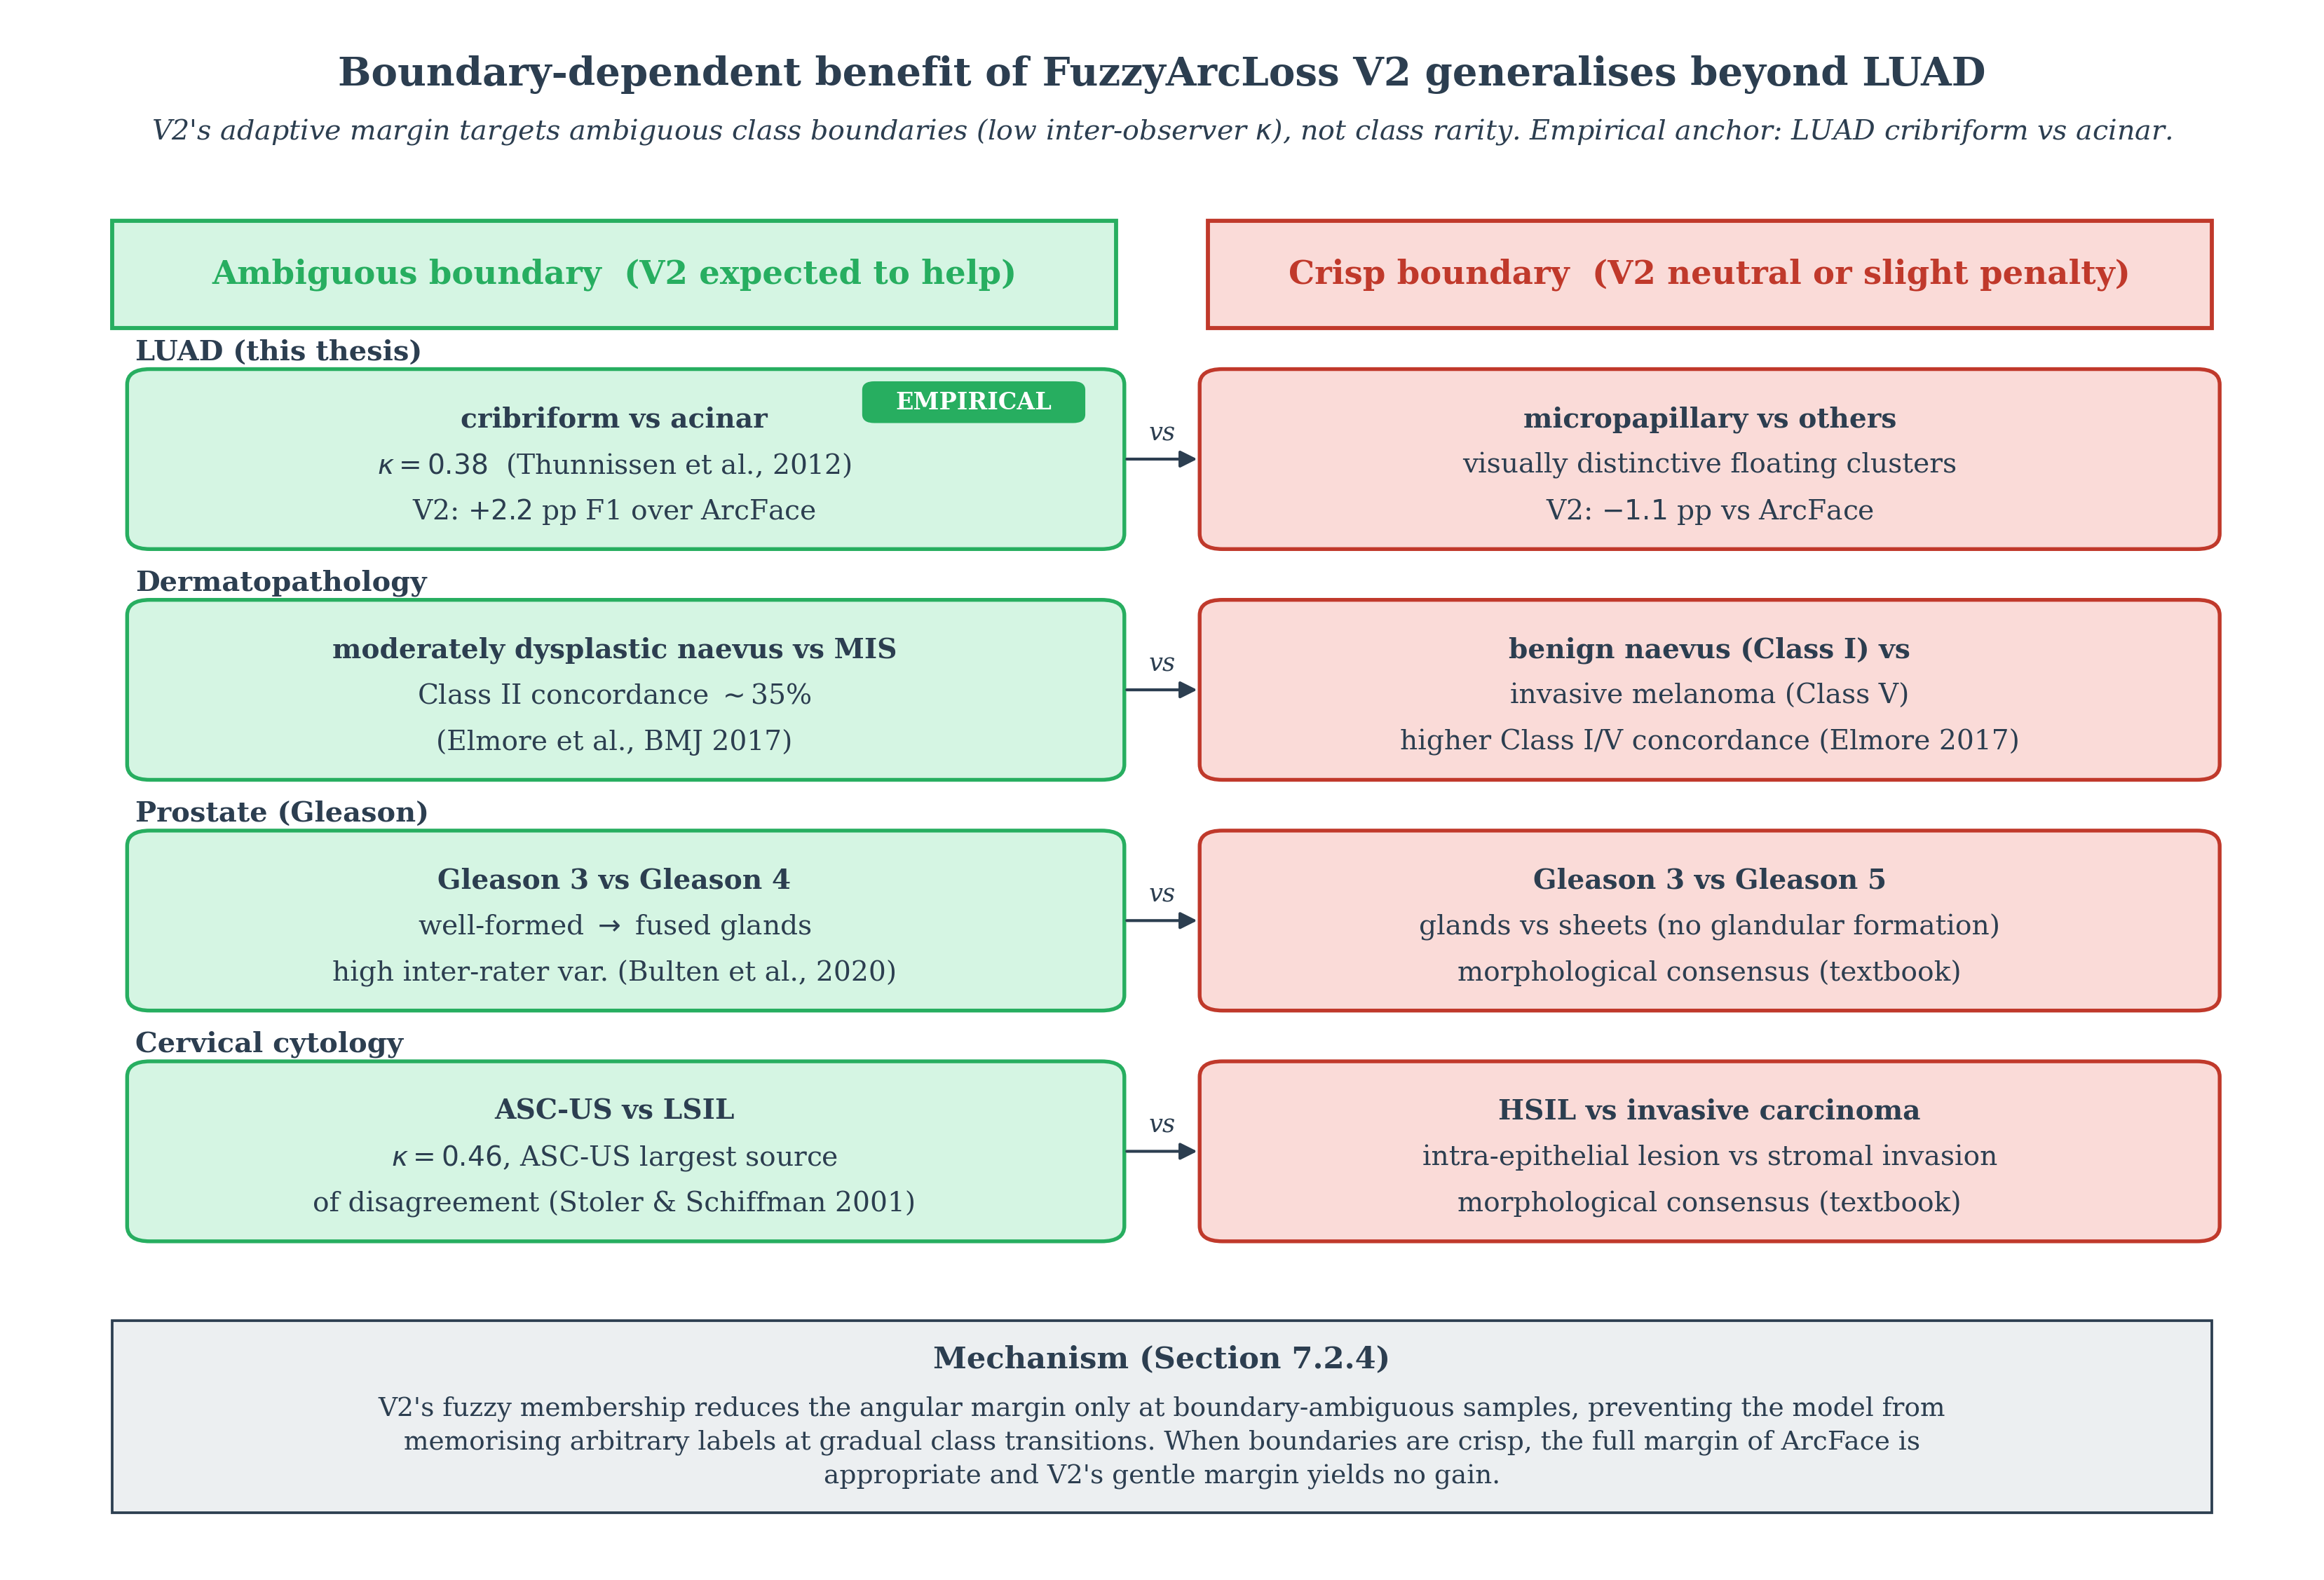
\includegraphics[width=\textwidth]{chapters/figures/boundary_dependent_generalization.png}
\caption[Boundary-dependent benefit of FuzzyArcLoss~V2 generalises beyond LUAD]{%
    Cross-domain projection of FuzzyArcLoss~V2's
    boundary-dependent advantage. Each row pairs an
    \emph{ambiguous} class boundary (left, green; with reported
    inter-observer agreement and source paper) with a
    \emph{crisp} class boundary (right, red; chosen as the
    visually distinctive contrast within the same diagnostic
    domain) so that the two compared classes share a common
    pathological context.
    Sources for the ambiguous-side claims:
    LUAD cribriform vs acinar
    ($\kappa = 0.38$,~\cite{thunnissen2012reproducibility}),
    Class~II MPATH-Dx melanocytic lesions
    ($\sim$35\% intraobserver concordance,~\cite{elmore2017melanoma}),
    Gleason 3 vs 4
    (high inter-rater variability,~\cite{bulten2020gleason}),
    ASC-US vs LSIL
    ($\kappa = 0.46$, ASC-US largest source of
    disagreement,~\cite{stoler2001alts}).
    The right-side ``crisp'' contrasts (Class~I/V melanocytic
    lesions, Gleason 3 vs 5, HSIL vs invasive carcinoma) are
    morphologically standard textbook contrasts within each
    domain (no specific reproducibility study cited; for melanoma
    Class~I/V the higher concordance is reported
    in~\cite{elmore2017melanoma} alongside Class~II).
    The LUAD row is empirical (cribriform vs acinar: $+2.2$\,pp
    over ArcFace, marked \textsc{empirical}; cf.\
    Figure~\ref{fig:boundary_vs_size}); the dermatopathology,
    prostate Gleason and cervical cytology rows are predictions
    under the boundary-dependence hypothesis. The bottom band
    states the underlying mechanism.}
\label{fig:boundary_dependent_generalization}
\end{figure}

% ============================================================================
\section{Limitations}
\label{sec:disc:limitations}
% ============================================================================

The limitations that bound the empirical claims of this thesis
fall into four classes; each is documented in detail in the
chapter where it was \emph{established}, so this section serves
primarily as a single-stop index pointing the reader to those
discussions, and reserves a full treatment only for the one
limitation that genuinely \emph{shapes} the conclusions and
therefore belongs in the discussion chapter:

\begin{itemize}
    \item \textbf{Implementation-time limitations} (residual GPU
    non-determinism: $\pm 0.8$\,pp single-run macro-F1 envelope;
    encoder choice: CTransPath~vs.\ UNI/RetCCL not benchmarked)
    are documented in
    Section~\ref{sec:impl:repro:limitations} of
    Chapter~\ref{ch:implementation}, alongside the engineering
    decisions that produced them.
    \item \textbf{Evaluation-design limitations} (single-cohort
    TCGA-LUAD, sample size $N=687$, ANORAK$\to$TCGA domain shift,
    preliminary single-pathologist validation, absence of spatial
    mutation ground truth, AUROC-vs-AUPRC ranking-bound limitation
    in the low-prevalence regime, uncalibrated probability
    outputs) are documented in the dedicated
    Section~\ref{sec:eval:limitations} of
    Chapter~\ref{ch:evaluation}, immediately adjacent to the
    experiments that revealed them; the per-class minority-class
    fragility (cribriform vs.\ micropapillary) is documented
    inline at Section~\ref{sec:eval:pattern:perclass}.
    \item \textbf{Methodological scope decisions}---no per-slide
    model arbitration (the system selects the best model per
    gene rather than per slide; the rationale is formalised in
    Section~\ref{sec:meth:interp:gene_vs_slide_selection}) and
    independent per-gene prediction without multi-task
    learning---are formalised in
    Chapter~\ref{ch:methodology}; their architectural relaxations
    (a learnable mixture-of-experts gate; a shared-encoder
    multi-task model with inter-gene Choquet aggregation) are
    developed in
    Section~\ref{sec:disc:future:medium} and need not be restated
    here.
\end{itemize}

The remaining limitation---a representational ceiling that follows
from the choice of \emph{label space} rather than from cohort,
metrics, or training---is the only one that directly \emph{shapes}
the analytical conclusions of this chapter, specifically the
RQ2(ii) ``no morphological projection'' mechanism of
Section~\ref{sec:disc:genotype_phenotype} and the boundary on
where any pattern representation can recover signal at all.
It is therefore developed in full below.

\subsection{Representational Ceiling: The Pattern Taxonomy as a
Pre-Committed Hypothesis Space}
\label{sec:disc:lim:method}

\textbf{Pattern taxonomy fixed at six output channels.}
The pattern classifier exposes a 6-dimensional categorical
output (a six-way softmax over the ANORAK label space:
lepidic, acinar, papillary, micropapillary, solid, cribriform),
which is the only label space for which an annotated training
set exists.
This output dimensionality is also a \emph{hard upper bound on
the information content} of the pattern channel: any
morphological feature outside the six-class vocabulary is, in
effect, an out-of-vocabulary token, by construction unreachable
for the downstream MIL aggregator regardless of how many slides
or how large a pretrained encoder is used.
Three biological features known to be prognostic in NSCLC fall
outside this vocabulary:
(i)~\emph{tumour budding}---small detached cell clusters
($\leq$5 cells) at the invasive front, encoding local cohesion
loss~\cite{kadota2015budding};
(ii)~\emph{tumour--stroma ratio (TSR)}---the
tumour-vs-stroma area fraction within a tile, a global
proportion-of-pixels feature~\cite{zhang2015tsr};
and (iii)~\emph{tumour-infiltrating lymphocyte (TIL) density}---a
spatial density map of lymphocytes inside and around the
tumour~\cite{brambilla2016til}.
Most consequential for this thesis is the absence of any
\emph{non-neoplastic} output channel (stroma, normal alveolar
parenchyma, immune compartment): the model has no representational
slot for the tumour microenvironment, so it cannot encode an
\emph{immune-cold} phenotype---an empirical regime in which TIL
density inside the tumour is at or near zero, robustly observed in
STK11-mutant LUAD and known to predict resistance to
immunotherapy~\cite{skoulidis2018stk11pd1}---even though that is
exactly the channel in which STK11's discriminative signal would
live.
The 6-pattern softmax is, in this sense, a pre-committed
hypothesis space rather than a free architectural choice, and
one that the present results show is not expressive enough for
genes whose discriminative signal lives outside it
(STK11, KEAP1, RBM10).


% ============================================================================
\section{Future Work}
\label{sec:disc:future}
% ============================================================================

The limitations documented in Section~\ref{sec:disc:limitations}
of this chapter and in the cross-referenced
Section~\ref{sec:impl:repro:limitations} of
Chapter~\ref{ch:implementation} and
Section~\ref{sec:eval:limitations} of
Chapter~\ref{ch:evaluation} directly suggest several directions
for future work, organised by time horizon.
Figure~\ref{fig:future_work_roadmap} provides a roadmap of the
items discussed in the three subsections that follow; each item
is annotated with the limitation it addresses.

\begin{figure}[ht!]
\centering
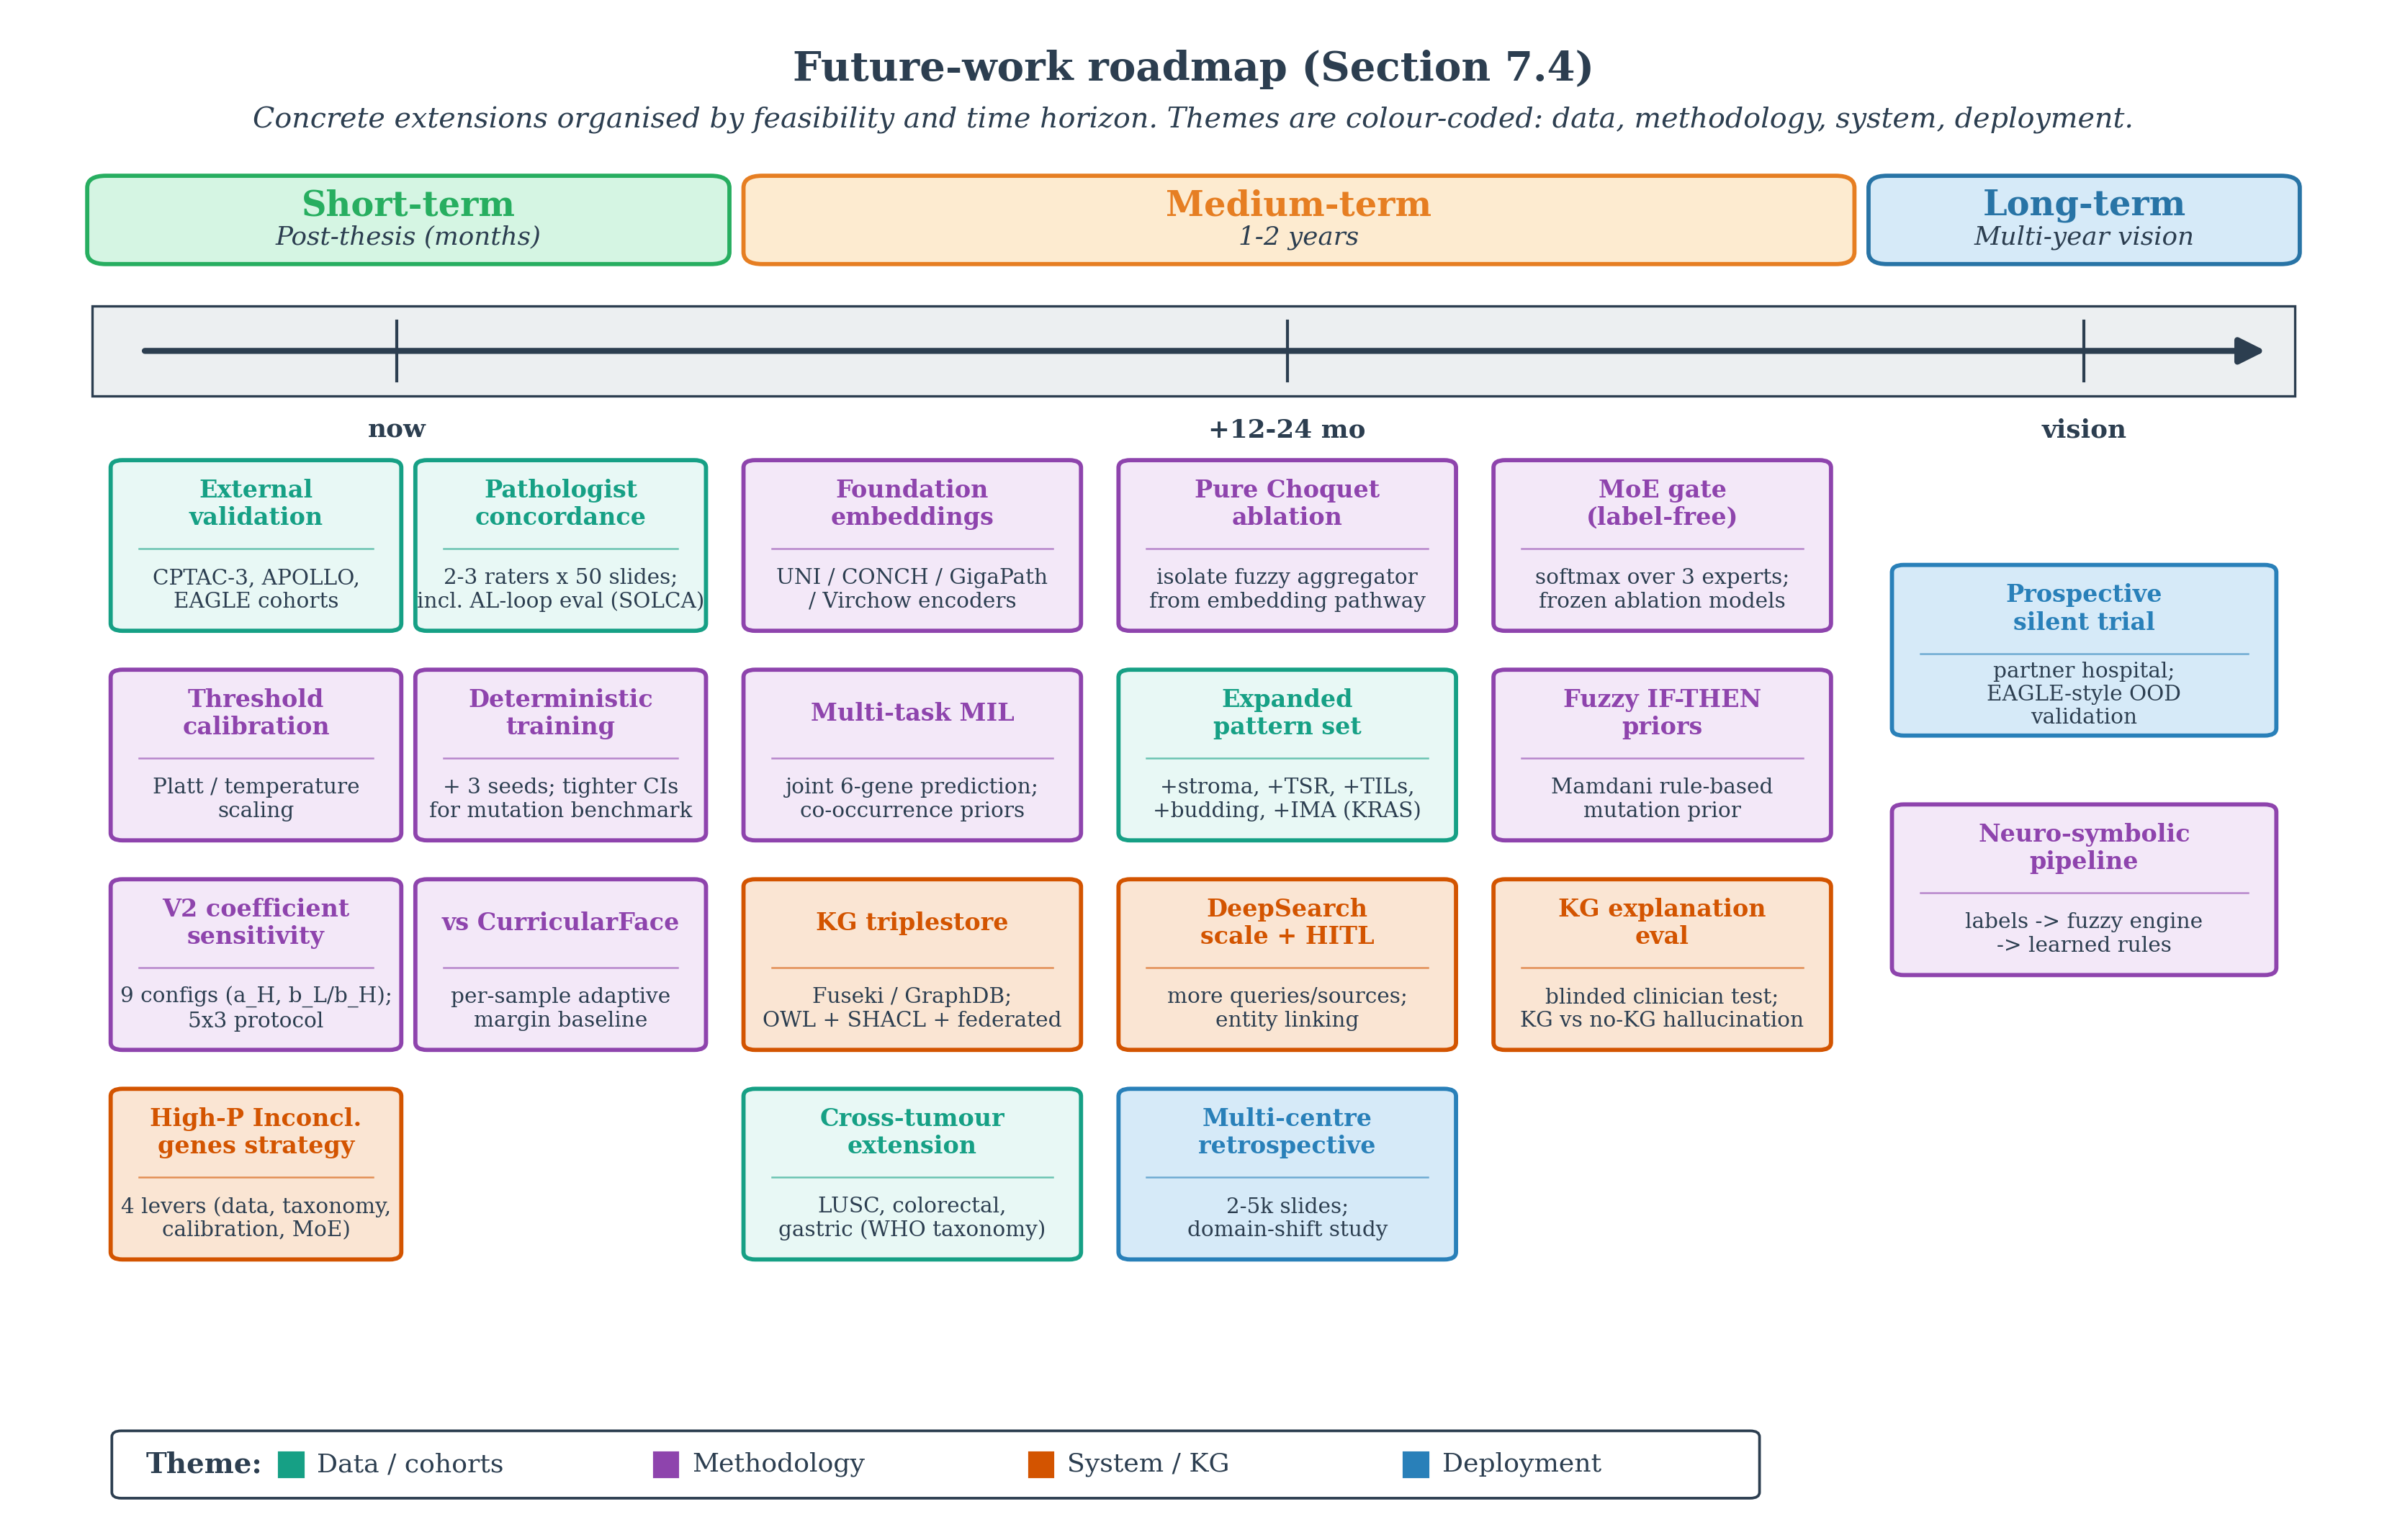
\includegraphics[width=\textwidth]{chapters/figures/future_work_roadmap.png}
\caption[Future-work roadmap]{%
    Three-tier roadmap of the future work discussed in
    Sections~\ref{sec:disc:future:short},
    \ref{sec:disc:future:medium}, and~\ref{sec:disc:future:long}.
    Cards are organised left to right by time horizon
    (post-thesis months $\to$ 1--2 years $\to$ multi-year vision)
    and colour-coded by theme: data and cohort extensions
    (teal), methodology (purple), system / knowledge graph
    (orange) and deployment / external validation (blue). Each
    card responds to a limitation documented in
    Section~\ref{sec:disc:limitations} (representational
    ceiling), Section~\ref{sec:eval:limitations}
    (data, calibration, AUROC-vs-AUPRC) or
    Section~\ref{sec:impl:repro:limitations}
    (engineering: non-determinism, encoder choice).}
\label{fig:future_work_roadmap}
\end{figure}

\subsection{Short-Term Extensions (Post-Thesis)}
\label{sec:disc:future:short}

\textbf{External validation on existing cohorts.}
\emph{Addresses the single-cohort evaluation limitation
(Section~\ref{sec:eval:lim:data}).}
The immediate, low-cost priority is to evaluate the
\emph{already-trained} TCGA-LUAD models on the three external
cohorts identified in Section~\ref{sec:uc:external}:
CPTAC-3 ($\sim$111 patients), APOLLO ($\sim$87), and EAGLE
($\sim$31).
This is a zero-retraining test that converts the thesis results
from single-cohort findings into multi-cohort evidence and is
distinct from the \emph{prospective scale-up} discussed under
medium-term work (Section~\ref{sec:disc:future:medium},
``Multi-centre retrospective studies''), which would re-train on
2{,}000--5{,}000 newly collected slides.

\textbf{Extended pathologist concordance study.}
\emph{Addresses the preliminary single-pathologist validation
limitation (Section~\ref{sec:eval:lim:data}).}
The preliminary review by a SOLCA pathologist
(Section~\ref{sec:eval:pattern:confusion}) established a baseline:
one expert evaluated eight subregions across five slides, revealing
domain shift and micropapillary--acinar confusion.
A natural extension is a formal multi-rater study in which 2--3
board-certified pathologists independently evaluate the LCHAI system
on 50 representative slides, measuring: (a)~inter-rater agreement
between pathologists and the pattern classifier, (b)~pathologist
confidence in the mutation predictions with and without the
six-level interpretability overlay, and (c)~time-to-decision for
mutation triage.
This study is the strongest candidate for a post-thesis publication.

\textbf{Threshold calibration and reliability characterisation.}
\emph{Addresses the uncalibrated-output limitation
(Section~\ref{sec:eval:lim:design}).}
Applying Platt or temperature scaling to the mutation outputs on a
held-out fold, together with a reliability-diagram analysis and an
\emph{extension} of the current AUROC-only Conclusive/Inconclusive
criterion to a prevalence-aware version that also incorporates
AUPRC, would close the calibration gap so that $P(\text{mut})$
can be read as a posterior probability.
Two caveats follow directly from
Section~\ref{sec:eval:lim:design} and must be stated to avoid
overpromising: probability calibration is \emph{ranking-invariant}
(it does not change AUROC) and does \emph{not} resolve the
AUPRC-vs-AUROC gap in the low-prevalence regime
(RBM10, $5.4\%$ prevalence; EGFR, $11.4\%$).
The four levers documented under ``Strategy for high-probability
Inconclusive genes'' below are the complementary mechanisms for
that residual gap.

\textbf{Deterministic training and seed-level repetition.}
\emph{Addresses the residual GPU non-determinism limitation
(Section~\ref{sec:impl:repro:limitations}).}
The mutation prediction benchmark currently runs five
patient-stratified folds with a single global seed and no
seed-level repetition, leaving the run-to-run non-determinism
of $\pm 0.8$\,pp documented in
Section~\ref{sec:impl:repro:limitations} unaveraged.
Enabling PyTorch's deterministic kernels at a documented
throughput cost, and repeating the 5-fold benchmark with 3 seeds
to match the $5 \times 3 = 15$-run pattern-classifier protocol of
Section~\ref{sec:eval:pattern:kfold}, would tighten the
per-condition CIs and---together with paired bootstrap
testing---enable formal statistical testing between mutation
prediction conditions.

\textbf{Empirical sensitivity sweep over the membership coefficients.}
The four coefficients of the FuzzyArcLoss~V2 piecewise membership
function ($a_H, b_H, a_L, b_L$) were derived analytically from
three design principles
(Section~\ref{sec:meth:pattern:fuzzyv2:membership}) and fixed
before the Optuna search over $s$, $m$ and $\tau$.
A nine-configuration grid varying $a_H \in \{0.7, 0.8, 0.9\}$ and
$b_L/b_H \in \{1, 2, 3\}$ under the existing 5-fold $\times$ 3-seed
protocol (135 runs total, feasible on the existing hardware) would
resolve whether the principled operating point is also data-driven
optimal.

\textbf{Direct comparison with CurricularFace.}
CurricularFace~\cite{huang2020curricularface} is the closest
related adaptive angular-margin loss
(Table~\ref{tab:margin_comparison}) and was deferred from the
present benchmark for the mechanism-mismatch reasons of
Section~\ref{sec:meth:pattern:fuzzyv2}.
The proposed short-term experiment is V2 vs CurricularFace under
a matched 15-run K-fold protocol on the 637-tile ANORAK split,
with CurricularFace's EMA momentum swept on a held-out fold; the
pre-registered hypothesis (Section~\ref{sec:disc:interp:fuzzy})
is that V2 retains its advantage on ambiguous-boundary classes
(cribriform, micropapillary) and ties on the visually distinctive
ones.

\textbf{Strategy for high-probability Inconclusive genes.}
A notable paradox is the gap between cohort AUROC and per-slide
$P(\text{mut})$: KRAS reaches $P(\text{mut}) = 0.965$ on
TCGA-55-7815 yet is labelled \emph{Inconclusive} because its
fold-level AUROC (0.609) is below the 0.70 threshold.
The paradox arises because AUROC measures population-level
ranking across all 687 slides whereas $P$ reflects the model's
confidence on a single, morphologically representative case.
Four levers could close this gap and are summarised visually in
Figure~\ref{fig:kras_inconclusive_strategies}:

\begin{description}
    \item[(i) Larger and more diverse cohorts.]
    Scaling to 2{,}000--5{,}000 slides from multiple institutions
    (long-term item; Section~\ref{sec:disc:future:medium}),
    particularly with the mucinous and IMA cases that are
    KRAS-predictive but under-represented in TCGA.
    \item[(ii) Expanded pattern taxonomy.]
    Adding a mucinous / IMA channel
    (Section~\ref{sec:disc:future:medium}, channel~(v) of the
    Expanded pattern taxonomy item) would give the Choquet
    aggregator the morphological feature most strongly tied to
    KRAS in the literature~\cite{shim2015krasmucinous}.
    Medium-term; requires new pixel-level annotations.
    \item[(iii) Per-slide confidence calibration.]
    A per-slide confidence score derived from morphological
    similarity to KRAS-positive training cases would flag
    individual slides such as TCGA-55-7815 as high-confidence
    even when the gene-level AUROC is Inconclusive.
    Reporting lever; short-term, conditional on a calibration set
    of pathologist-validated representative slides per gene
    (Section~\ref{sec:eval:lim:data}).
    \item[(iv) Per-slide model selection.]
    A learnable mixture-of-experts gate over the Level~5 ablation
    panel could route each slide to its expected best model.
    Inference-time lever; calibrating without circularity on
    $N = 687$ slides is the blocker.
    Detailed in Section~\ref{sec:disc:future:moe_gate}.
\end{description}

\begin{figure}[ht!]
\centering
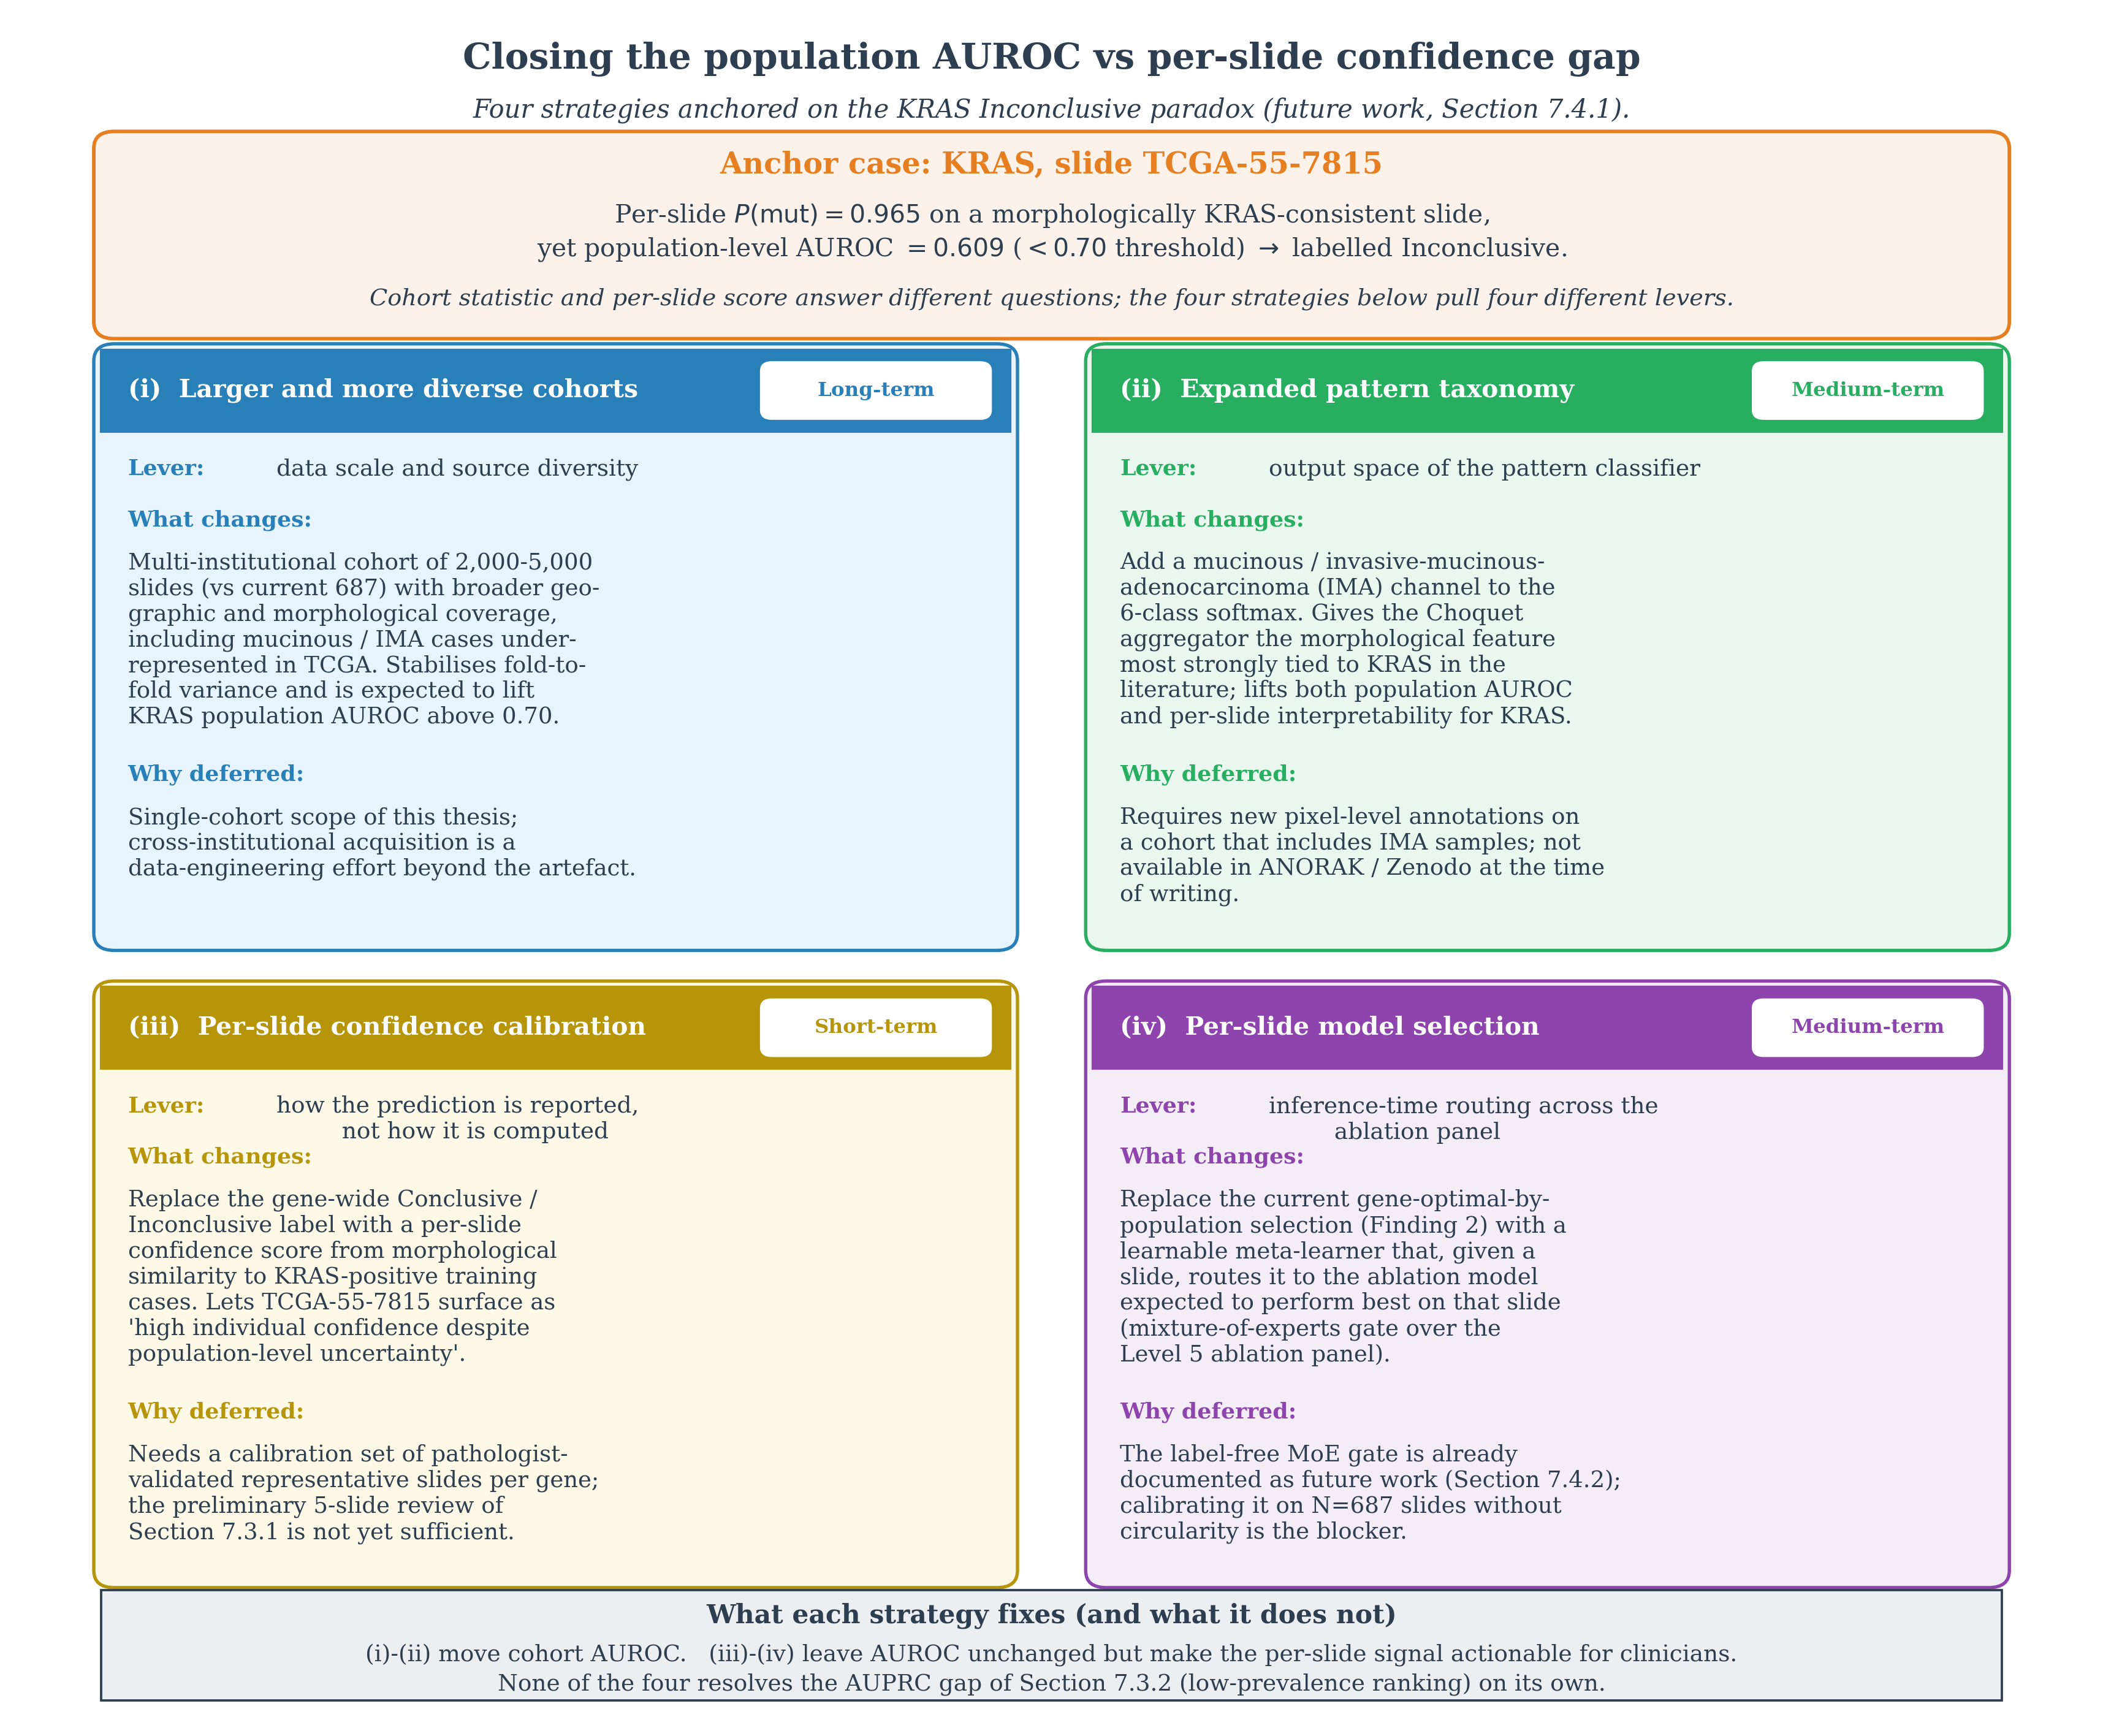
\includegraphics[width=\textwidth]{chapters/figures/kras_inconclusive_strategies.png}
\caption[Four strategies for closing the population AUROC vs
per-slide confidence gap]{%
    Four strategies for closing the population AUROC vs
    per-slide confidence gap, anchored on the KRAS Inconclusive
    paradox (TCGA-55-7815: per-slide $P(\text{mut})=0.965$ on a
    morphologically KRAS-consistent slide, yet
    population-level AUROC $=0.609<0.70$ threshold).
    The four strategies act on independent levers (data scale,
    output space, reporting, inference-time routing).
    Strategies (i) and (ii) move the cohort AUROC, while (iii)
    and (iv) leave AUROC unchanged but make the per-slide signal
    actionable for clinicians.
    None of the four resolves the AUPRC gap discussed in
    Section~\ref{sec:eval:lim:design} (low-prevalence ranking)
    on its own.}
\label{fig:kras_inconclusive_strategies}
\end{figure}

\subsection{Medium-Term Extensions (1--2 Years)}
\label{sec:disc:future:medium}

\textbf{Foundation model embeddings.}
\emph{Addresses the encoder-substitution limitation
(Section~\ref{sec:impl:repro:limitations}).}
Replacing CTransPath with more recent encoders
(UNI, CONCH, GigaPath, Virchow~\cite{chen2024uni,xu2024gigapath})
tests whether the pattern-informed approach still adds value on
top of embeddings optimised across diverse histopathology tasks.
Persistence of the KRAS Choquet lift (lepidic$\times$solid
synergy) under a stronger encoder would be strong evidence that
the fuzzy aggregation captures encoder-independent inter-pattern
structure; RBM10's FC-MIL behaviour is the negative control
(empty Choquet branch; Section~\ref{sec:eval:interp:choquet}).

\textbf{Dedicated Choquet-only ablation.}
The current FC-MIL is dual-pathway (CTransPath embeddings +
Choquet branch on pattern memberships).
A pure Choquet model on pattern probabilities alone would isolate
the aggregation mechanism and clarify whether KRAS's Choquet
advantage is interaction-driven and whether RBM10's apparent lift
is fully embedding-driven (Section~\ref{sec:eval:interp:choquet}).

\textbf{Slide-level mixture-of-experts gate for label-free model arbitration.}
\label{sec:disc:future:moe_gate}
\emph{Addresses the no-per-slide-arbitration scope decision
(Chapter~\ref{ch:methodology},
Section~\ref{sec:meth:interp:gene_vs_slide_selection}; index in
Section~\ref{sec:disc:limitations}).}
Section~\ref{sec:meth:interp:gene_vs_slide_selection} of
Chapter~\ref{ch:methodology} formalises why LCHAI~v2.0 fixes the
prediction model at the gene level rather than per slide:
runtime per-slide selection requires the ground-truth label,
the sigmoid outputs of independently trained ablation models are
not directly comparable as probabilities, and na\"{\i}ve
$\max$-of-experts is not generally a better classifier than the
per-gene best-in-expectation model.
A principled relaxation is a learnable mixture-of-experts gate
$g_\theta(\mathbf{x})$ that maps a slide's features to a convex
combination over the three frozen ablation predictors,
\[
P_{\text{gated}}
= \alpha_{\text{B2}} P_{\text{emb}}
+ \alpha_{\text{PI}} P_{\text{comb}}
+ \alpha_{\text{B3}} P_{\text{pat}},
\]
trained on input features only (no test labels) under the same
5-fold protocol of Chapter~\ref{ch:evaluation}.
Slides such as TCGA-49-AAR9 (KEAP1) and TCGA-49-AAR0 (STK11),
where Level~5 ablation already reveals a clear
$\Delta_{\text{pat}}$ signal, would be the natural test cases.
The expected gain is an empirical question against the per-gene
baseline of Table~\ref{tab:mutation_luad}, and the construction
must avoid the post-hoc cherry-picking ruled out in
Section~\ref{sec:meth:interp:gene_vs_slide_selection}.

\textbf{Multi-task and multi-gene learning.}
\emph{Addresses the independent-per-gene-prediction scope
decision (index in Section~\ref{sec:disc:limitations};
mechanism~4 of Section~\ref{sec:disc:genotype_phenotype}).}
The current artefact predicts six genes as independent binaries,
discarding the structured co-occurrence
(Section~\ref{sec:disc:genotype_phenotype}, mechanism~4).
A multi-task ABMIL with a shared encoder and six gene-specific
heads trained under a joint multi-label objective with a small
label-correlation regulariser is the natural extension; the
Choquet aggregation generalises symmetrically to inter-gene
interactions, exposing learnable Shapley values and pairwise
indices that mirror known co-occurrence structure (e.g., the
KRAS--STK11 immune-cold
pair~\cite{skoulidis2018stk11pd1}) and provide the empirical
test that mechanism~(4) actually constrains single-gene
predictions.

\textbf{Expanded pattern taxonomy (output-space extension).}
\emph{Addresses the representational-ceiling limitation
(Section~\ref{sec:disc:lim:method}).}
The pattern classifier's representational capacity is bounded by
its 6-way softmax (Section~\ref{sec:disc:lim:method}); enlarging
the output space is therefore a direct lever on the information
content of the pattern channel.
Concretely, this means re-training the tile classifier with
additional output channels for features that the current
ontology cannot express:
(i)~a \emph{non-neoplastic} class (stroma, normal alveolar
parenchyma) that lets the model expose tissue context outside the
tumour itself;
(ii)~a \emph{tumour--stroma ratio} regression head that exposes
the relative areas of tumour and stroma at the tile level;
(iii)~a \emph{lymphocyte-density} channel that quantifies
tumour-infiltrating lymphocytes (TILs) per tile;
(iv)~a \emph{tumour-budding} channel for small cell clusters
at the invasive edge;
and (v)~a \emph{mucinous / invasive mucinous adenocarcinoma (IMA)}
channel that expresses the architectural feature most strongly
tied to KRAS in the
literature~\cite{shim2015krasmucinous,rekhtman2013krassolid}---
the WHO~2021 IMA category that the present 6-channel ANORAK
ontology does not represent and that drives KRAS into the
``cross-term in label space'' regime of Finding~2
(Section~\ref{sec:disc:future:short}, lever~(ii)).
Adding (i) and (iii) is the most consequential change for STK11:
they together expose the immune-microenvironment axis where the
``immune-cold'' phenotype~\cite{skoulidis2018stk11pd1} lives,
lifting STK11 out of the RQ2(ii) ``no morphological projection''
regime that bounded its performance in this thesis.
Channel~(v) is the analogous lever for KRAS: a dedicated mucinous
basis vector removes the need for FC-MIL to recover IMA as a
lepidic--solid AND-conjunction
(Section~\ref{sec:eval:interp:choquet}).
Channels~(ii) and~(iv) target finer-grained signal known to carry
prognostic information but currently unrepresentable in the
6-pattern simplex.


\textbf{Fuzzy rule-based mutation priors (symbolic prior on top
of the neural pipeline).}
A complementary direction to the learned 2-additive measure of
FC-MIL is an explicit Mamdani-style fuzzy inference
system~\cite{mamdani1975experiment} whose IF--THEN rules encode
published pattern--gene associations
(e.g., \texttt{IF} \texttt{solid\_pct} \texttt{IS high} \texttt{AND}
\texttt{micropapillary\_pct} \texttt{IS medium} \texttt{THEN}
\texttt{TP53\_risk} \texttt{IS elevated}).
The defuzzified output of the rule base would be concatenated
with the slide-level neural representation as an additional
feature, giving a hybrid neuro-symbolic predictor in which the
symbolic prior is fully readable, validatable, and editable by a
domain expert without retraining.

\paragraph{Ontology and knowledge graph extension.}
The current knowledge graph is a curated edge store with NCIt/MONDO
IRIs plus a PostgreSQL table for DeepSearch-discovered relations
(Section~\ref{sec:meth:ontology:sparql}); migrating to a formal
triplestore (Apache Jena Fuseki or GraphDB) with a SPARQL endpoint
would unlock OWL reasoning over transitive associations, SHACL
shape validation at ingestion, and federated queries against the
EBI RDF platform and NCI Thesaurus SPARQL service.
The codebase already includes a SPARQL backend that can query
Fuseki and is disabled by default.
Integrating additional ontologies (DOID, SNOMED~CT, ICD-O) is the
natural follow-up.

\paragraph{DeepSearch scaling and validation.}
The current pipeline processes 12 curated queries
(Table~\ref{tab:deepsearch_queries}) against three literature
sources; scaling queries and sources, strengthening entity
linking (currently dictionary-based), and adding HITL review of
discovered relations before ingestion would raise reliability and
coverage of the enrichment layer.

\paragraph{Explainability evaluation (LLM agent, KG, reader
study).}
\emph{Addresses the explainability-not-evaluated limitation.}
This thesis evaluates LCHAI's \emph{interpretability}
empirically in Chapter~\ref{ch:evaluation} at two
levels: per-slide (six-level inspection framework, intrinsic
Choquet Shapley values, on representative TCGA cases) and
per-gene at the cohort level (Conclusive/Inconclusive
reliability flag from the held-out 5-fold AUROC, Hosmer--Lemeshow
threshold $\geq 0.70$).
Its \emph{explainability}---the natural-language rationales produced
by the KG-grounded LLM agent---is claimed only as a system
capability and is not formally evaluated
(Section~\ref{sec:bg:xai:definitions}).
Three complementary evaluations would close this gap:
(i)~\textbf{Faithfulness audit}---automated check that every
clinical claim in an LLM explanation is supported by the
underlying interpretability outputs (attention map, pattern
overlay, SHAP/Choquet values, KG triple), with a measurable
unsupported-claim rate;
(ii)~\textbf{KG correctness and coverage}---a curated
pattern\,$\to$\,gene\,$\to$\,treatment gold standard plus a
blinded clinician comparison of LLM explanations with vs.\ without
KG grounding to quantify hallucination reduction;
(iii)~\textbf{Reader study}---blinded pathologists rate
explanation utility, completeness and clinical accuracy on
representative true-positive and false-negative slides, including
a calibration check that prediction probabilities are invariant
to enabling or disabling the KG layer (the KG is downstream of
prediction by design).
 

\textbf{Pipeline transferability beyond LUAD.}
The three-artefact pipeline (fuzzy margin classification $\to$
pattern-informed MIL $\to$ Choquet aggregation) is parameterised
on the pattern label space rather than on lung adenocarcinoma
specifically: the only LUAD-specific component is the 6-way ANORAK
softmax that defines the input simplex of the Choquet branch.
The pipeline therefore transfers, with no architectural change, to
any tumour type for which a fixed pattern taxonomy and a
tile-level annotated training set are available---candidates
include lung squamous cell carcinoma (LUSC), colorectal
adenocarcinoma, and gastric cancer, all of which have
established growth-pattern taxonomies in the WHO classification
of tumours.
Replicating the present evaluation on a second tumour type would
test whether the boundary-dependent benefit of FuzzyArcLoss~V2 and
the inter-pattern interaction modelling of FC-MIL generalise
beyond LUAD, and would provide a broader evidence base for
fuzzy representation learning in computational pathology.

\textbf{Multi-centre retrospective studies (prospective scale-up).}
\emph{Addresses the limited-sample-size limitation
(Section~\ref{sec:eval:lim:data}); orthogonal to the
zero-retraining external validation of
Section~\ref{sec:disc:future:short}.}
Where the short-term external-validation item tests the
\emph{already-trained} TCGA-LUAD models on existing public
cohorts (CPTAC-3, APOLLO, EAGLE), this medium-term item is a
distinct effort to \emph{re-train and re-evaluate} on
2{,}000--5{,}000 newly collected slides from multiple institutions,
which would reduce fold-to-fold variance and enable more powerful
statistical comparisons between conditions.


\subsection{Long-Term Vision}
\label{sec:disc:future:long}

\textbf{Out-of-distribution deployment validation (prospective
clinical study).}
The ultimate generalisation test is to evaluate LCHAI on a
prospective stream of incoming cases at a partner hospital---a
fully out-of-distribution setting in which scanner, staining
protocol and patient demographics differ from the TCGA
training cohort, and in which the system runs without ever
seeing the ground-truth label until after the prediction is
made (silent-trial protocol).
EAGLE~\cite{campanella2025eagle} demonstrates that this regime
is achievable for an EGFR predictor, reaching AUROC~$0.890$ on
197 patients and projecting a $43\%$ reduction in unnecessary
molecular testing.
The present work does not approach that scale, but it
contributes the interpretable framework within which such a
deployment can be designed---with the practical difference that
clinicians can audit and override the model's reasoning
slide-by-slide via the pattern overlay and the six-level XAI
stack, rather than treating the predictor as an opaque
classifier whose only failure signal is a wrong probability.

\textbf{Fuzzy neuro-symbolic mutation prediction.}
A longer-term research direction is the development of a fully neuro-symbolic pipeline in which the pattern classifier provides symbolic labels (``solid,'' ``acinar''), the fuzzy logic engine reasons over these labels using domain-encoded rules and learned fuzzy measures, and the neural network provides the visual backbone.
This architecture would maximise interpretability while maintaining the flexibility of deep learning, representing a principled synthesis of the fuzzy and neural paradigms.


% ============================================================================
\section{Conclusion}
\label{sec:disc:conclusion}

Table~\ref{tab:rq_summary_ch7} summarises the status of each research
question.

\begin{table}[ht!]
\centering
\small
\caption[Summary of research question outcomes]{Summary of
research question outcomes
(Section~\ref{sec:eval:rq}).
Quantitative evidence and contribution mapping are reported
separately in Table~\ref{tab:contribution_finding_map}
(Section~\ref{sec:disc:contributions})
to keep the two tables orthogonal.}
\label{tab:rq_summary_ch7}
\renewcommand{\arraystretch}{1.15}
\begin{tabularx}{\textwidth}{@{}c X X@{}}
\hline
\textbf{RQ} & \textbf{Core question} & \textbf{Outcome} \\
\hline
1     & Adaptive fuzzy loss improves pattern classification?       & Met \\
2(i)  & Pattern-informed MIL improves cohort-level AUROC?          & Partially met (gene-dependent) \\
2(ii) & Three-regime, five-mechanism ontology-coverage taxonomy?   & Met \\
3     & Fuzzy Choquet captures inter-pattern interactions?         & Met \\
4     & Clinically meaningful explanations?                        & Met \\
5     & Domain knowledge competitive under data scarcity?          & Met (greater-benefit-under-scarcity untested) \\
6     & Ontology-grounded explanations?                            & Met \\
7     & DeepSearch produces validated candidate relations?         & Met \\
\hline
\end{tabularx}
\end{table}

This thesis investigated pattern-informed fuzzy deep learning for
interpretable genotype--phenotype inference in lung adenocarcinoma
under the constraint of limited public data.
Three computational artefacts (FuzzyArcLoss~V2, Pattern-Informed
ABMIL, Fuzzy Choquet MIL) and a fourth ontology-grounded
explanation layer were developed and evaluated within the Design
Science Research framework, and were composed into the LCHAI~v2.0
prototype; the detailed contribution-to-evidence mapping is in
Table~\ref{tab:contribution_finding_map} and the empirical results
are in Chapter~\ref{ch:evaluation}.
At matched public-data scale the system is statistically
comparable to the strongest peer studies on the two clinically
actionable genes (TP53, EGFR) while providing interpretability
none of them offer; the gap to foundation-scale proprietary
studies is structural (data asymmetry,
Section~\ref{sec:eval:literature}), not methodological.

\textbf{Three analytical takeaways.}
The empirical chapters yield three analytical takeaways, ordered
chronologically by the artefact and evaluation stage in which each
emerged.

\emph{Takeaway~1 (Artefact~1, pattern classification,
Section~\ref{sec:eval:pattern:perclass}).}
FuzzyArcLoss~V2's advantage is
\emph{morphological-boundary-dependent, not
class-size-dependent}: the relevant ``boundary'' is the
\emph{decision surface between adjacent histological pattern
classes}, and the fuzzy-margin mechanism helps wherever that
surface is genuinely gradual---i.e., where the two classes
overlap visually and inter-annotator agreement is low---rather
than wherever a class has few training samples
(Section~\ref{sec:eval:pattern:perclass} contrasts cribriform and
micropapillary at identical class size to demonstrate the
dissociation).
This is a transfer rule that generalises beyond LUAD to Gleason
grading, Pap-smear cytology and dermatopathology
(Section~\ref{sec:disc:interp:fuzzy};
Figure~\ref{fig:boundary_dependent_generalization}).

\emph{Takeaway~2 (Artefacts~2 and~3, mutation prediction,
Section~\ref{sec:disc:interp:domain}).}
Fuzzy logic earns its keep only when applied \emph{coherently}
across training, representation and aggregation, and only when
the target gene's biology lives in inter-pattern co-occurrence:
the pattern prior beats a strong pretrained encoder solely on
KRAS, where Choquet aggregation recovers the
lepidic$\times$solid synergy that proxies the missing
invasive-mucinous class
(Section~\ref{sec:disc:interp:domain}).
This refines, rather than confirms, the common ``small model
with domain prior beats large encoder'' narrative.

\emph{Takeaway~3 (cross-gene synthesis,
Section~\ref{sec:disc:genotype_phenotype}).}
Aggregating across the six target genes, the underlying learning
problem is fundamentally \textbf{stochastic, many-to-many and
weakly labelled}, not a deterministic morphology-to-genotype
function: label noise is structural, gene-by-gene heterogeneity
is the rule, and competence has to be argued per gene and per
representative slide rather than declared from a single AUROC
(Section~\ref{sec:disc:genotype_phenotype}).

Together, these three takeaways constitute the analytical
contribution that connects the formalism of fuzzy set theory to
the biology of cancer genomics.

\textbf{Interpretability matters most where the predictor is
wrong.}
The representative-case analysis
(Section~\ref{sec:eval:interp:enrichment}) shows that on true
positives the explanation pathway is merely confirmatory, but on
the four false negatives it is \emph{decisive}: it distinguishes
a confidently-negative prediction from a signal-absent one---a
distinction the raw probability cannot make---and surfaces, slide
by slide, which failure mode of the taxonomy the case exhibits.
The cohort-level Conclusive/Inconclusive flag is genuinely
\emph{independent} of this per-slide signal: three of the four
false-negative genes (STK11, KEAP1, RBM10) are also Inconclusive,
but EGFR is Conclusive at the cohort level yet false-negative on
its representative slide---the case that proves the two layers
are complementary rather than redundant.
No prior H\&E mutation predictor exposes both layers, making this
the strongest interpretability contribution of the artefact
stack.

\textbf{Verdict on the central hypothesis.}
The hypothesis (Section~\ref{sec:intro:hypothesis}) is
\emph{partially supported}: fuzzy-encoded domain knowledge
achieves mutation-prediction performance competitive with the
public-data literature while enabling a six-level
interpretability framework absent from all prior work.
The support is \emph{partial} in two specific senses:
\begin{itemize}
    \item \textbf{Gene-conditional.}
    The pattern-prior lift over a strong pretrained encoder
    appears only on KRAS, where Choquet aggregation recovers
    the lepidic$\times$solid synergy that proxies the missing
    invasive-mucinous adenocarcinoma class.
    On TP53 and EGFR the encoder already saturates the
    morphological signal (Regime~A); on STK11, KEAP1 and
    RBM10 the discriminative signal lies outside the
    6-pattern simplex altogether (Regime~B).
    \item \textbf{Aggregator-conditional.}
    Even on KRAS, the lift requires FC-MIL's Choquet integral.
    Linear concatenation (PI-ABMIL) cannot represent the
    inter-pattern AND-conjunction and collapses; pattern-only
    streams (B3) underperform without the embedding pathway
    (Regime~C).
\end{itemize}

The companion \emph{three-mechanism ontology-coverage taxonomy}
of RQ2(ii) (Section~\ref{sec:eval:rq2}) names the three
structural reasons a 6-channel pattern simplex can fail to
recover a mutation signal:
\emph{label-space mismatch} (terminology imported from domain
adaptation~\cite{lipton2018labelshift}; instantiated by
STK11---signal in the tumour microenvironment, outside the
ANORAK label set);
\emph{no morphological projection} (term original to this
thesis, grounded in biology~\cite{li2011keap1papillary};
instantiated by KEAP1---upstream oxidative-stress pathway
with no H\&E correlate); and
\emph{collapse-to-prior} (terminology imported from
variational inference~\cite{bowman2016posteriorcollapse};
instantiated by RBM10---low prevalence traps every channel at
the base rate).
The taxonomy is therefore an \emph{empirical} contribution
with mixed pedigree: two of the three names are imports
adapted from neighbouring fields, the third is original to
this thesis, and applying the resulting three-way taxonomy to
TCGA-LUAD with the ANORAK simplex bounds what any pattern-only
representation can recover
(Figure~\ref{fig:signal_tree}).
This refines, rather than refutes, the hypothesis.

\textbf{Principal claims and final position.}
The six fine-grained \emph{contributions}~C1--C6 enumerated in
Section~\ref{sec:disc:contributions}
(Table~\ref{tab:contribution_finding_map};
Figure~\ref{fig:contribution_evidence_map}) are the
deliverables of the thesis; they support two
\emph{principal claims} that are what the thesis ultimately
defends.
Artefacts C1--C4 and the ontology explanation layer C6
collectively support the methodological claim, and the
gene-by-gene taxonomy C5 supports the analytical claim.
The principal claims of this thesis are therefore not
clinical-grade mutation prediction---foundation-scale 60{,}000+
slide cohorts already exist for that purpose---but the
following two:
\begin{enumerate}
    \item \textbf{Claim~(i) --- methodological
    (supported by C1--C4 + C6).}
    Fuzzy logic, applied coherently across loss
    (\emph{C1}), representation (\emph{C2}) and aggregation
    (\emph{C3}), makes a public-data prediction pipeline
    transparent through a six-level interpretability stack
    integrated in the LCHAI~v2.0 prototype (\emph{C4}) and
    grounded in an NCIt/MONDO knowledge graph with literature
    enrichment (\emph{C6}).
    \item \textbf{Claim~(ii) --- empirical/analytical
    (supported by C5).}
    The three-regime taxonomy enunciated above bounds what any
    morphology-only model can achieve from H\&E alone, and
    identifies the genes for which fusing additional data
    sources (gene-expression profiles, radiology), rather than
    further architectural refinement, is the natural next step.
\end{enumerate}
The approach does not compete with the brute-force scaling of
foundation models but offers a complementary paradigm: one in
which a pathologist can understand, verify and \emph{correct} the
model's reasoning, and in which interpretability is most valuable
precisely on the cases the predictor gets wrong.
As computational pathology moves from research prototypes toward
clinical deployment, the ability to explain predictions---and to
explain failures---in terms that clinicians recognise may prove
as important as the predictions themselves.